\documentclass[12pt,a4paper]{report}

% ---------------------------------------------------------
% Packages & Environment Setup
% ---------------------------------------------------------
\usepackage[utf8]{inputenc}
\usepackage[margin=1in]{geometry}
\usepackage{amsmath,amssymb,amsfonts}
\usepackage{graphicx}
\usepackage{xcolor}
\usepackage{hyperref}
\usepackage{booktabs}
\usepackage{multirow}
\usepackage{listings}
\usepackage{caption}
\usepackage{subcaption}
\usepackage{fancyhdr}
\usepackage{tcolorbox}
\usepackage{tikz}
\usetikzlibrary{shapes.geometric, arrows.meta, positioning, shadows}

% ---------------------------------------------------------
% Formatting & Color Definitions
% ---------------------------------------------------------
\definecolor{primaryblue}{RGB}{21, 101, 192}
\definecolor{darknavy}{RGB}{27, 42, 61}
\definecolor{accentcyan}{RGB}{0, 172, 193}
\definecolor{codebg}{RGB}{245, 247, 250}
\definecolor{codecomment}{RGB}{100, 116, 139}

\hypersetup{
    colorlinks=true,
    linkcolor=primaryblue,
    filecolor=primaryblue,      
    urlcolor=primaryblue,
    citecolor=primaryblue
}

\lstset{
    backgroundcolor=\color{codebg},
    basicstyle=\ttfamily\footnotesize,
    breaklines=true,
    captionpos=b,
    commentstyle=\color{codecomment},
    keywordstyle=\color{primaryblue}\bfseries,
    stringstyle=\color{accentcyan},
    frame=single,
    rulecolor=\color{lightgray}
}

% tcolorbox setup for User Guide Note Boxes
\tcbuselibrary{skins,breakable}
\newtcolorbox{guidebox}[2][]{
    colback=white,
    colframe=primaryblue,
    fonttitle=\bfseries\color{white},
    title=#2,
    enhanced,
    attach boxed title to top left={xshift=3mm,yshift=-3mm},
    boxed title style={colback=primaryblue},
    #1
}

% ---------------------------------------------------------
% DOCUMENT START
% ---------------------------------------------------------
\begin{document}

\setcounter{chapter}{3} % Sets this as Chapter 4
\chapter{Integration and Platform}
\label{chap:integration_and_platform}

\section{Introduction and Overview}
Modern cellular telecommunication networks rely on two distinct engineering disciplines: \textbf{Radio Access Network (RAN) Optimization} and \textbf{5G Network Parameter Planning}. Historically, these domains operated in isolated software tools, creating workflow fragmentation and data silos between Optimization Engineers troubleshooting operational degraded drive-test paths and Planning Engineers allocating physical cell parameters for new and existing gNodeB base stations.

This chapter presents the design, architecture, implementation, and feature breakdown of the \textbf{NetFix Unified RAN \& 5G Planning Platform}—the primary software deliverable of this graduation project. The platform integrates two independent microservice ecosystems into a single, cohesive, enterprise-grade React 19 web application:
\begin{enumerate}
    \item \textbf{Drive-Test Analytics \& Anomaly Detection Portal (NetFix):} A multi-stage statistical, Machine Learning (Histogram Gradient Boosting), and PyTorch LSTM temporal fusion platform coupled with a deterministic 34-reason cause-matching engine and local LLM diagnostic narrative generation.
    \item \textbf{5G New Radio (NR) Planning Portal (NetPulse):} A spatial geometry, neighbor graph, and constraint satisfaction engine for allocating Physical Cell Identifiers (PCI), Root Sequence Indices (RSI), and PRACH parameters while enforcing strict modulo (Mod3, Mod4, Mod30) conflict rules.
\end{enumerate}

The platform enforces a strict \textbf{Role-Based Access Control (RBAC)} and forwarding model. Upon authentication, users are automatically routed to their specialized engineering environment while retaining access to an interactive workspace switcher.

\subsection{Technology Stack Specification}
The platform combines modern web development frameworks, asynchronous Python backend microservices, specialized machine learning engines, persistent document stores, and zero-cloud local AI runtimes. Table~\ref{tab:tech_stack} outlines the complete technology stack.

\begin{table}[htbp]
\centering
\caption{NetFix Unified Platform Complete Technology Stack Specification.}
\label{tab:tech_stack}
\small
\begin{tabular}{lllp{7cm}}
\toprule
\textbf{Layer / Tier} & \textbf{Technology / Library} & \textbf{Version} & \textbf{Role \& Functional Scope} \\
\midrule
\multirow{6}{*}{\textbf{Presentation}} 
 & React & 19.0 & Core reactive component frontend framework. \\
 & TypeScript & 5.5 & Strict static type checking and payload contracts. \\
 & Vite & 5.4 & High-performance frontend build engine \& HMR. \\
 & Tailwind CSS & 4.0 & Modern utility-first styling with dark mode themes. \\
 & Leaflet GIS & 1.9.4 & High-performance map canvas for GPS breadcrumbs. \\
 & Recharts / Plotly.js & 2.12 / 2.29 & Interactive time-series \& severity chart rendering. \\
\midrule
\multirow{4}{*}{\textbf{Orchestration}} 
 & FastAPI & 0.110 & Asynchronous REST API orchestrator (Python 3.11). \\
 & Uvicorn & 0.28 & High-concurrency ASGI web server implementation. \\
 & Pydantic & 2.6 & Data validation, setting management, schema definitions. \\
 & HTTPX & 0.27 & Async HTTP client for inter-service RPC proxying. \\
\midrule
\multirow{4}{*}{\textbf{ML \& Analytics}} 
 & PyTorch & 2.2 & Sequence windowing \& PyTorch LSTM temporal prediction. \\
 & Scikit-Learn & 1.4 & Histogram Gradient Boosting ($Q_{50}, Q_{75}$) regressors. \\
 & NumPy / Pandas & 1.26 / 2.2 & High-throughput vectorized matrix \& data frame operations. \\
 & OpenPyXL & 3.1 & Parsing and generation of cellular \texttt{.xlsx} workbooks. \\
\midrule
\multirow{2}{*}{\textbf{Data \& Cache}} 
 & MongoDB & 7.0 & Document database for sessions, telemetry, and rules. \\
 & Redis & 7.2 & In-memory cache for RCA incident caching and locks. \\
\midrule
\textbf{AI Runtime} 
 & Ollama Local LLM & 0.1.28 & Isolated container running local \texttt{llama3.1} \& \texttt{deepseek-r1}. \\
\bottomrule
\end{tabular}
\end{table}

---

\section{System Architecture and Integration Model}

\subsection{Architectural Blueprint}
The platform architecture adopts a decoupled microservice paradigm orchestrated via Docker Compose. The software stack consists of five core tiers:
\begin{itemize}
    \item \textbf{Presentation Tier (Unified Web UI):} Built with React 19, TypeScript, Vite, Tailwind CSS v4, Leaflet GIS maps, and Recharts. Serves as the single pane of glass for both planning and optimization workflows.
    \item \textbf{Orchestration Tier (NetFix FastAPI Backend):} Implements a two-phase Analysis Session state machine that sequences raw data ingestion, feature generation, anomaly pipeline execution, threshold evaluation, and AI diagnostic generation.
    \item \textbf{Execution Engine Tier (Python Microservices):} Modular execution containers housing the 11-stage drive-test cleaning pipeline (\texttt{ran-cleaning-service}), 19-stage anomaly detection engine (\texttt{ran-anomaly-service}), and 5G constraint engine (\texttt{planning-backend}).
    \item \textbf{Data Tier (MongoDB 7.0 \& Redis):} Persistent document storage housing raw session summaries, spatial cell handoffs, anomaly shortlist incidents, and the 34-reason cellular degradation taxonomy.
    \item \textbf{Local AI Runtime Tier (Ollama Engine):} Isolated container running local quantized LLM models (\texttt{llama3.1}, \texttt{deepseek-r1:8b}) and embedding models (\texttt{nomic-embed-text}) for zero-cloud API dependency.
\end{itemize}

\begin{figure}[htbp]
\centering
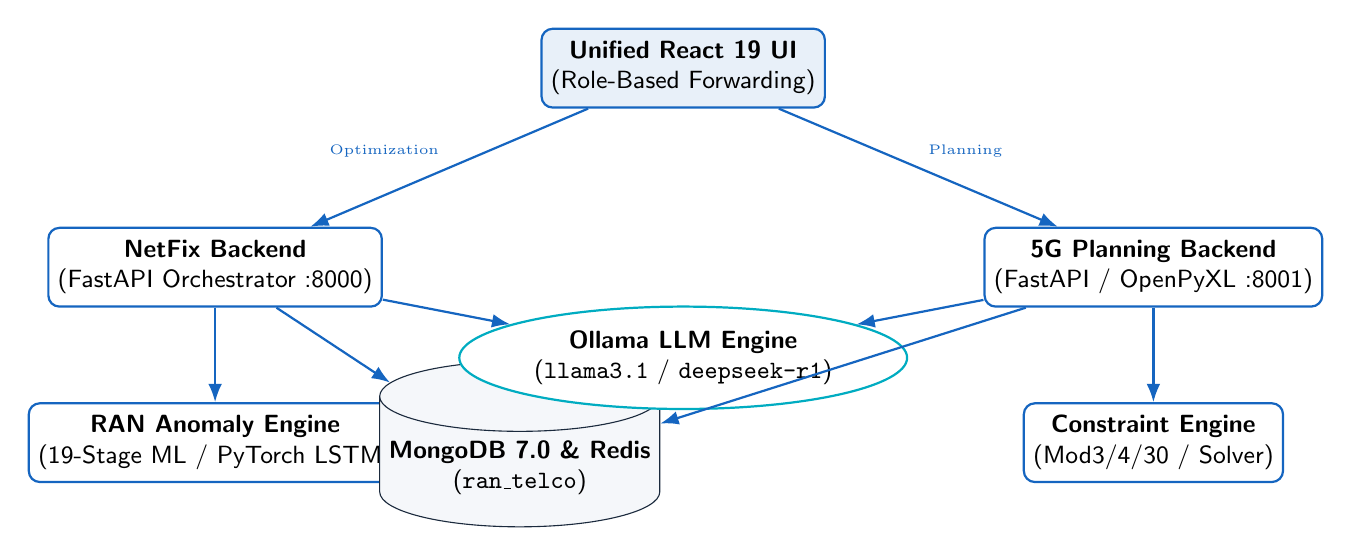
\begin{tikzpicture}[
    node distance=1.5cm and 2cm,
    block/.style={rectangle, draw=primaryblue, fill=white, rounded corners, thick, align=center, minimum width=3cm, minimum height=1cm, font=\sffamily\small},
    dbblock/.style={cylinder, draw=darknavy, fill=codebg, shape border rotate=90, aspect=0.25, align=center, minimum width=2.5cm, minimum height=1.2cm, font=\sffamily\small},
    cloudblock/.style={ellipse, draw=accentcyan, fill=white, thick, align=center, minimum width=2.5cm, minimum height=1cm, font=\sffamily\small},
    arrow/.style={-Latex, thick, primaryblue}
]
    % Nodes
    \node[block, fill=primaryblue!10] (ui) {\textbf{Unified React 19 UI}\\(Role-Based Forwarding)};
    \node[block, below left=of ui] (anomaly_be) {\textbf{NetFix Backend}\\(FastAPI Orchestrator :8000)};
    \node[block, below right=of ui] (plan_be) {\textbf{5G Planning Backend}\\(FastAPI / OpenPyXL :8001)};
    \node[block, below=1.2cm of anomaly_be] (anomaly_engine) {\textbf{RAN Anomaly Engine}\\(19-Stage ML / PyTorch LSTM)};
    \node[block, below=1.2cm of plan_be] (plan_engine) {\textbf{Constraint Engine}\\(Mod3/4/30 / Solver)};
    \node[dbblock, below right=0.8cm and 0.5cm of anomaly_be] (mongo) {\textbf{MongoDB 7.0 \& Redis}\\(\texttt{ran\_telco})};
    \node[cloudblock, below=2.5cm of ui] (ollama) {\textbf{Ollama LLM Engine}\\(\texttt{llama3.1} / \texttt{deepseek-r1})};

    % Paths
    \draw[arrow] (ui) -- node[above left, font=\tiny]{Optimization} (anomaly_be);
    \draw[arrow] (ui) -- node[above right, font=\tiny]{Planning} (plan_be);
    \draw[arrow] (anomaly_be) -- (anomaly_engine);
    \draw[arrow] (plan_be) -- (plan_engine);
    \draw[arrow] (anomaly_be) -- (mongo);
    \draw[arrow] (plan_be) -- (mongo);
    \draw[arrow] (anomaly_be) -- (ollama);
    \draw[arrow] (plan_be) -- (ollama);
\end{tikzpicture}
\caption{Overall Platform Microservice Architecture and Inter-Service Communications.}
\label{fig:platform_architecture}
\end{figure}

\subsection{Dynamic Multi-Port Backend Probing Mechanism}
To seamlessly unify two independent backends without port collisions during container deployment, the frontend implements a dynamic probing resolution mechanism (\texttt{src/netpulse/api.ts}):
\begin{lstlisting}[language=TypeScript, caption={Dynamic Multi-Port Resolution Helper in Frontend API Client.}]
const PLANNING_BACKEND_CANDIDATES = [
  'http://localhost:8001',
  'http://localhost:8000'
];

async function fetchFromPlanningBackend(endpoint: string, options?: RequestInit) {
  for (const baseUrl of PLANNING_BACKEND_CANDIDATES) {
    try {
      const response = await fetch(`${baseUrl}${endpoint}`, options);
      if (response.ok || response.status === 422) return response;
    } catch (e) {
      // Continue probing next port candidate
    }
  }
  throw new Error(`Failed to connect to Planning Backend service.`);
}
\end{lstlisting}
This allows the \textbf{NetFix Anomaly Backend} to operate on host port \texttt{8000} and the \textbf{NetPulse 5G Planning Backend} on host port \texttt{8001}, while ensuring failover support if deployed in single-port proxy configurations.

\subsection{Two-Phase Analysis Session Lifecycle State Machine}
To prevent expensive computational re-execution of ML models when engineers adjust KPI thresholds, data processing follows a persistent \textbf{Two-Phase State Machine}:

\begin{table}[htbp]
\centering
\caption{Two-Phase Analysis Session State Transitions.}
\label{tab:session_state_machine}
\small
\begin{tabular}{lllp{6cm}}
\toprule
\textbf{State Transition} & \textbf{Trigger Event} & \textbf{Execution Duration} & \textbf{Computed Artifacts \& Storage} \\
\midrule
\texttt{CREATED} $\rightarrow$ \texttt{PHASE1\_RUNNING} & Pickle file upload & Instant & Raw dataframe received; session document created in MongoDB. \\
\texttt{PHASE1\_RUNNING} $\rightarrow$ \texttt{PHASE1\_DONE} & Data cleaning \& ML fitting & $10$--$30$ seconds (One-time) & Runs 11-stage cleaning, z-scores, HGB regressors, PyTorch LSTM. Stores candidate incident JSONs. \\
\texttt{PHASE1\_DONE} $\rightarrow$ \texttt{PHASE2\_RUNNING} & Threshold tuning submission & $<1$ second (Interactive) & Evaluates RSRP/RSRQ/SINR/BLER threshold labels on cached data. \\
\texttt{PHASE2\_RUNNING} $\rightarrow$ \texttt{PHASE2\_DONE} & Rule matching \& LLM invoke & $1$--$3$ seconds & Matches 34-reason condition catalog, executes Redis caching, prompts Ollama narrative. \\
\bottomrule
\end{tabular}
\end{table}

\subsection{Database Schema \& Document Structure}
The platform utilizes MongoDB collection schemas inside the \texttt{ran\_telco} database:
\begin{table}[htbp]
\centering
\caption{MongoDB Database Collection Specifications.}
\label{tab:mongo_collections}
\small
\begin{tabular}{llp{8cm}}
\toprule
\textbf{Collection Name} & \textbf{Primary Key} & \textbf{Contents \& Description} \\
\midrule
\texttt{analysis\_sessions} & \texttt{session\_id} & Master session summary, upload metadata, threshold state, matched cause dicts, and LLM text summaries. \\
\texttt{rca\_reasons} & \texttt{reason\_id} & 34-reason cellular degradation graph containing categories, preconditions, and recommended actions. \\
\texttt{rca\_anomaly\_incidents\_full\_compact} & \texttt{incident\_id} & Full list of candidate anomaly incidents with spatial, statistical, and ML features. \\
\texttt{rca\_anomaly\_incidents\_shortlist\_diverse} & \texttt{incident\_id} & High-priority operational anomaly shortlist after spatial-temporal deduplication. \\
\texttt{worst\_performing\_cells\_rca\_handoff} & \texttt{cell\_id} & Aggregated KPI statistics and failure counts grouped by ECI cell identifiers. \\
\texttt{worst\_performing\_pci\_rca\_handoff} & \texttt{pci} & Aggregated KPI statistics and handoff counts grouped by Physical Cell Identity. \\
\bottomrule
\end{tabular}
\end{table}

\subsection{Role-Based Authentication and Dynamic Routing}
The platform implements client-side and server-side role evaluation logic. Users register with explicit engineering roles which govern initial portal forwarding:

\begin{equation}
\text{ForwardingTarget}(\text{Role}) = 
\begin{cases} 
\text{5G Planning Portal (\texttt{/np-upload})}, & \text{if } \text{Role} \text{ contains ``Planning''} \\
\text{Anomaly Detection Portal (\texttt{/dashboard})}, & \text{otherwise}
\end{cases}
\end{equation}

---

\section{Deep Feature Breakdown: Anomaly Detection and RCA Platform}

\subsection{11-Stage Data Cleaning Pipeline (\texttt{ran-cleaning-service})}
Raw drive-test datasets (\texttt{.pkl}) undergo sequential cleaning across 11 non-leaking stages:
\begin{itemize}
    \item \textbf{Stage 01--04 (Settings \& Utility Helpers):} Configures headless Matplotlib execution (\texttt{Agg}), sets environment output paths, and loads spatial-temporal utility helpers.
    \item \textbf{Stage 05--06 (Raw Data Load \& Profiling):} Loads pickle payloads, profiles missing value ratios, inspects coordinate integrity (Latitude/Longitude), and establishes a cleaning plan.
    \item \textbf{Stage 07--08 (Feature Derivation \& Throughput Detection):} Derives movement speed (km/h), temporal windowing variables, and dynamically detects LTE Downlink throughput KPI columns.
    \item \textbf{Stage 09--11 (Filtering, Aliasing \& Quality Bins):} Applies LTE-DL record filtering, generates neighbor cell aggregate statistics, computes event-window spatial rolling means, and formats quality flags.
\end{itemize}

\subsection{19-Stage Multi-Model Anomaly Fusion Engine (\texttt{ran-anomaly-service})}
Anomaly detection combines robust statistical baselines, supervised machine learning, and deep sequence modeling:
\begin{enumerate}
    \item \textbf{Robust Statistical Scores (Stages 01--04):} Computes cell-level z-scores using Median Absolute Deviation (MAD):
    \begin{equation}
    Z_{\text{MAD}} = \frac{x_i - \text{median}(X)}{1.4826 \cdot \text{MAD}(X)}, \quad \text{where } \text{MAD}(X) = \text{median}(|X - \text{median}(X)|)
    \end{equation}
    Calculates group-based P75 expected throughput fallback hierarchies (Cell P75 $\rightarrow$ RB-conditioned P75 $\rightarrow$ Global P75).
    
    \item \textbf{Machine Learning Cross-Fitting (Stages 08--11):} Performs out-of-fold cross-fitted prediction using Scikit-Learn's \texttt{HistGradientBoostingRegressor} under Pinball Quantile Loss:
    \begin{equation}
    \mathcal{L}_q(y, \hat{y}) = \max\Big(q(y - \hat{y}), (q-1)(y - \hat{y})\Big)
    \end{equation}
    evaluating expected resource throughput ($Q_{50}$ and $Q_{75}$).
    
    \item \textbf{PyTorch LSTM Sequence Models (Stages 12--14):} Constructs sliding temporal sequence windows ($W = 10$ steps) and trains a PyTorch recurrent neural network:
    \begin{equation}
    h_t = \tanh(W_{hh} h_{t-1} + W_{xh} x_t + b_h)
    \end{equation}
    generating out-of-fold temporal throughput predictions ($LSTM \text{-} Q_{50}$).
    
    \item \textbf{Row-Level Anomaly Fusion Layer (Stage 16):} Combines statistical deviations, ML quantile residuals, and PyTorch LSTM temporal errors into a composite anomaly score:
    \begin{equation}
    \text{Score}_{\text{Fused}} = w_1 \cdot Z_{\text{Stat}} + w_2 \cdot \frac{|\text{TP}_{\text{Actual}} - \text{TP}_{\text{HGB}}|}{\text{TP}_{\text{Expected}}} + w_3 \cdot \frac{|\text{TP}_{\text{Actual}} - \text{TP}_{\text{LSTM}}|}{\text{TP}_{\text{Expected}}}
    \end{equation}
    
    \item \textbf{Operational Incident Deduplication (Stages 17--19):} Clusters candidate spatial-temporal anomaly points into distinct candidate episodes, filters strict RCA episodes, and exports shortlist incident JSON artifacts.
\end{enumerate}

\subsection{KPI Threshold Evaluation and Labeling Bins}
Network telemetry metrics are evaluated against customizable operator threshold bins:
\begin{itemize}
    \item \textbf{RSRP (Reference Signal Received Power):} Good ($> -90$ dBm), Acceptable ($-105$ to $-90$ dBm), Poor ($< -105$ dBm).
    \item \textbf{RSRQ (Reference Signal Received Quality):} Good ($> -10$ dB), Acceptable ($-15$ to $-10$ dB), Poor ($< -15$ dB).
    \item \textbf{SINR (Signal-to-Interference-plus-Noise Ratio):} Good ($> 13$ dB), Acceptable ($0$ to $13$ dB), Poor ($< 0$ dB).
    \item \textbf{BLER (Block Error Rate):} Good ($< 5\%$), Acceptable ($5\%$ to $10\%$), Poor ($> 10\%$).
\end{itemize}

\subsection{Deterministic Rule Engine \& 34-Reason Degradation Taxonomy}
Unlike unreliable generative-only models, root cause matching is \textbf{100\% deterministic}. The system evaluates the anomaly's labeled KPI vector against an explicit condition catalog (\texttt{rules/condition_catalog.py}) representing 34 cellular failure modes, including:
\begin{itemize}
    \item \texttt{coverage\_hole}: RSRP is Poor, RSRQ is Poor, SINR is Poor.
    \item \texttt{high\_bler\_dl}: Downlink BLER is Poor ($>10\%$) while RSRP is Acceptable or Good.
    \item \texttt{rb\_congestion}: High Physical Resource Block (PRB) usage with low achieved throughput despite clean RF conditions.
    \item \texttt{pilot\_pollution}: Multiple strong serving/neighbor PCI signals with low SINR ($<0$ dB) despite adequate RSRP.
    \item \texttt{mimo\_rank\_fallback}: High SINR ($>15$ dB) accompanied by anomalous Rank 1 transmission mode.
\end{itemize}

\subsection{AI Diagnostic Narrative Generator (Local Ollama LLM)}
Once root cause matching identifies candidate failure reasons, the backend invokes a local LLM (\texttt{llama3.1} or \texttt{deepseek-r1:8b} via Ollama) to synthesize a plain-language diagnostic report consisting of:
\begin{enumerate}
    \item Executive Problem Summary.
    \item Root Cause Narrative explaining physical RF degradation mechanisms.
    \item Key Supporting KPI Evidence Bullet Points.
    \item Recommended Actionable Mitigation Steps (e.g., tilt adjustments, power control tweaks, parameter corrections).
\end{enumerate}

---

\section{Deep Feature Breakdown: 5G NR Planning Platform}

\subsection{5G Parameter Allocation Domain}
The 5G Planning Portal manages Physical Cell Identifiers (PCI $\in [0, 1007]$), Primary Sync Signals ($PSS = PCI \pmod 3$), Secondary Sync Signals ($SSS = \lfloor PCI / 3 \rfloor$), Demodulation Reference Signals ($DMRS = PCI \pmod 4$), and Root Sequence Indices ($RSI \in [0, 837]$) for Physical Random Access Channels (PRACH).

\subsection{Spatial Neighbor Graph \& Azimuth Geometry}
The constraint engine (\texttt{pipeline/neighbor_graph.py}) computes spatial topology:
\begin{itemize}
    \item \textbf{Spatial Distance Matrix:} Calculates pairwise Haversine distances between all base station sites:
    \begin{equation}
    d = 2R \arcsin \left( \sqrt{\sin^2\left(\frac{\Delta \phi}{2}\right) + \cos(\phi_1)\cos(\phi_2)\sin^2\left(\frac{\Delta \lambda}{2}\right)} \right)
    \end{equation}
    \item \textbf{Azimuth Bounding \& Overlap:} Evaluates sector orientation angles ($\theta_{\text{azimuth}}$) and beam overlap angles to establish directional neighbor pairs.
    \item \textbf{Forbidden Set Computation:} Calculates a set of forbidden PCIs/RSIs for candidate sectors based on active neighbor allocations within spatial threshold radius $D_{\text{threshold}}$.
\end{itemize}

\subsection{Inter-Cell Modulo Clash Detection Engine}
The validation engine (\texttt{pipeline/validator.py}) audits networks for hard and soft clashes:
\begin{table}[htbp]
\centering
\caption{5G NR Modulo Clash Definitions and Failure Criteria.}
\label{tab:mod_clashes}
\small
\begin{tabular}{lllp{6cm}}
\toprule
\textbf{Clash Type} & \textbf{Category} & \textbf{Rule Condition} & \textbf{Engineering Impact} \\
\midrule
\textbf{PCI Co-Channel} & Hard (Must be 0) & $PCI_A = PCI_B, d < D_{\text{reuse}}$ & Direct signal collision and call drop. \\
\textbf{PCI Confusion} & Hard (Must be 0) & $PCI_B = PCI_C$ for neighbors of $A$ & Target cell identification ambiguity during handover. \\
\textbf{Mod3 Clash} & Soft / Warning & $PCI_A \pmod 3 = PCI_B \pmod 3$ & PSS reference signal sequence interference. \\
\textbf{Mod4 Clash} & Hard (Must be 0) & $PCI_A \pmod 4 = PCI_B \pmod 4$ & Cell-specific RS and DMRS symbol position collision. \\
\textbf{Mod30 Clash} & Soft / Warning & $PCI_A \pmod {30} = PCI_B \pmod {30}$ & SSS and DMRS sequence pattern overlap. \\
\textbf{RSI Collision} & Hard (Must be 0) & $RSI_A = RSI_B, d < D_{\text{PRACH}}$ & False preamble detection and PRACH channel blocked. \\
\bottomrule
\end{tabular}
\end{table}

\subsection{Constraint Satisfaction Replanning Engine (CSP)}
The planning backend implements a global greedy constraint satisfaction solver (\texttt{bulk\_plan.py}) that assigns non-clashing PCI and RSI values across all sector nodes:
\begin{enumerate}
    \item Construct spatial neighbor adjacency list $G = (V, E)$ using Haversine distance threshold $D_{\text{threshold}} = 5.0$ km.
    \item For each sector node $v_i \in V$, compute active forbidden set $F(v_i)$:
    \begin{equation}
    F(v_i) = \bigcup_{(v_i, v_j) \in E} \{ \text{PCI}(v_j) \} \cup \{ p \mid p \pmod 4 = \text{PCI}(v_j) \pmod 4 \}
    \end{equation}
    \item Select candidate assignment $p^* \in [0, 1007] \setminus F(v_i)$ that minimizes soft Mod3 and Mod30 penalties.
    \item Update network state dynamically and output updated \texttt{.xlsx} workbook.
\end{enumerate}

\subsection{Grounded Tool-Calling AI Assistant (\texttt{OCTO})}
The planning portal incorporates \texttt{OCTO}, a tool-calling AI assistant (\texttt{agent.py}). All calculations (neighbor distance, candidate PCI valid lists, clash counts) are executed by underlying Python functions, ensuring the AI model never hallucinates engineering calculations.

---

\section{User Guide: NetFix Anomaly Detection and RCA Portal}

\begin{guidebox}{Target Persona: Optimization Engineer / RF Performance Specialist}
This user guide provides an exhaustive, step-by-step operational manual for Radio Access Network (RAN) Optimization Engineers. Grounded strictly in actual UI screenshots of the \textbf{NetFix Anomaly Detection Portal}, this document details every navigation module, KPI widget, pipeline progress stepper, deterministic root-cause breakdown, GIS map interface, and interactive AI Copilot workflow.
\end{guidebox}

\subsection{System Navigation and Portal Layout Framework}
The NetFix interface is structured around a persistent dark-navy primary navigation sidebar (\texttt{\#1B2A3D}) and an enterprise light workspace area (\texttt{\#F8FAFC}):
\begin{enumerate}
    \item \textbf{NETFIX ANALYSIS Module Group:}
    \begin{itemize}
        \item \textbf{Dashboard:} Real-time overall telemetry health overview, KPI metric cards, severity distributions, and high-resolution ML backend time-series figures.
        \item \textbf{Upload Dataset:} Ingestion dropzone for raw \texttt{.pkl} network drive-test payloads with 4-stage execution stepper and recent session audit log.
        \item \textbf{Results:} Root Cause Analysis (RCA) engine, 23-metric telemetry breakdown grids, 3GPP standard references, and vendor resolution steps.
        \item \textbf{Interactive Map:} High-performance Leaflet GIS canvas plotting drive-test GPS breadcrumbs, cell towers, and pinpoint anomaly markers.
    \end{itemize}
    \item \textbf{INSIGHTS Module Group:}
    \begin{itemize}
        \item \textbf{Reports:} Automated PDF diagnostic summaries and exported data profiling figures.
        \item \textbf{Penguin AI:} Conversational AI Engineering Copilot powered by local quantized LLMs (\texttt{llama3.1}, \texttt{deepseek-r1}) for deep technical reasoning and grounded report generation.
    \end{itemize}
    \item \textbf{SYSTEM Module Group:}
    \begin{itemize}
        \item \textbf{History:} Audit log tracking all historical analysis sessions, completion statuses, anomaly counts, and cause-matching totals.
        \item \textbf{Settings:} Threshold configuration defaults, model selection preferences, and API endpoints.
    \end{itemize}
    \item \textbf{User Context Badge (Bottom-Left):} Displays logged-in engineer credentials (\texttt{Mego 312002}, \texttt{Optimization Eng.}), active role badge, and session logout controls.
\end{enumerate}

---

\subsection{Module 1: Telemetry Overview \& ML Pipeline Dashboard}
\textit{Reference Screenshot: \texttt{Screenshot from 2026-08-12 14-38-38.png}}

The \textbf{Dashboard} view serves as the primary operational landing page after portal authentication. It consolidates dataset-wide telemetry metrics and machine learning validation plots:

\begin{figure}[htbp]
\centering
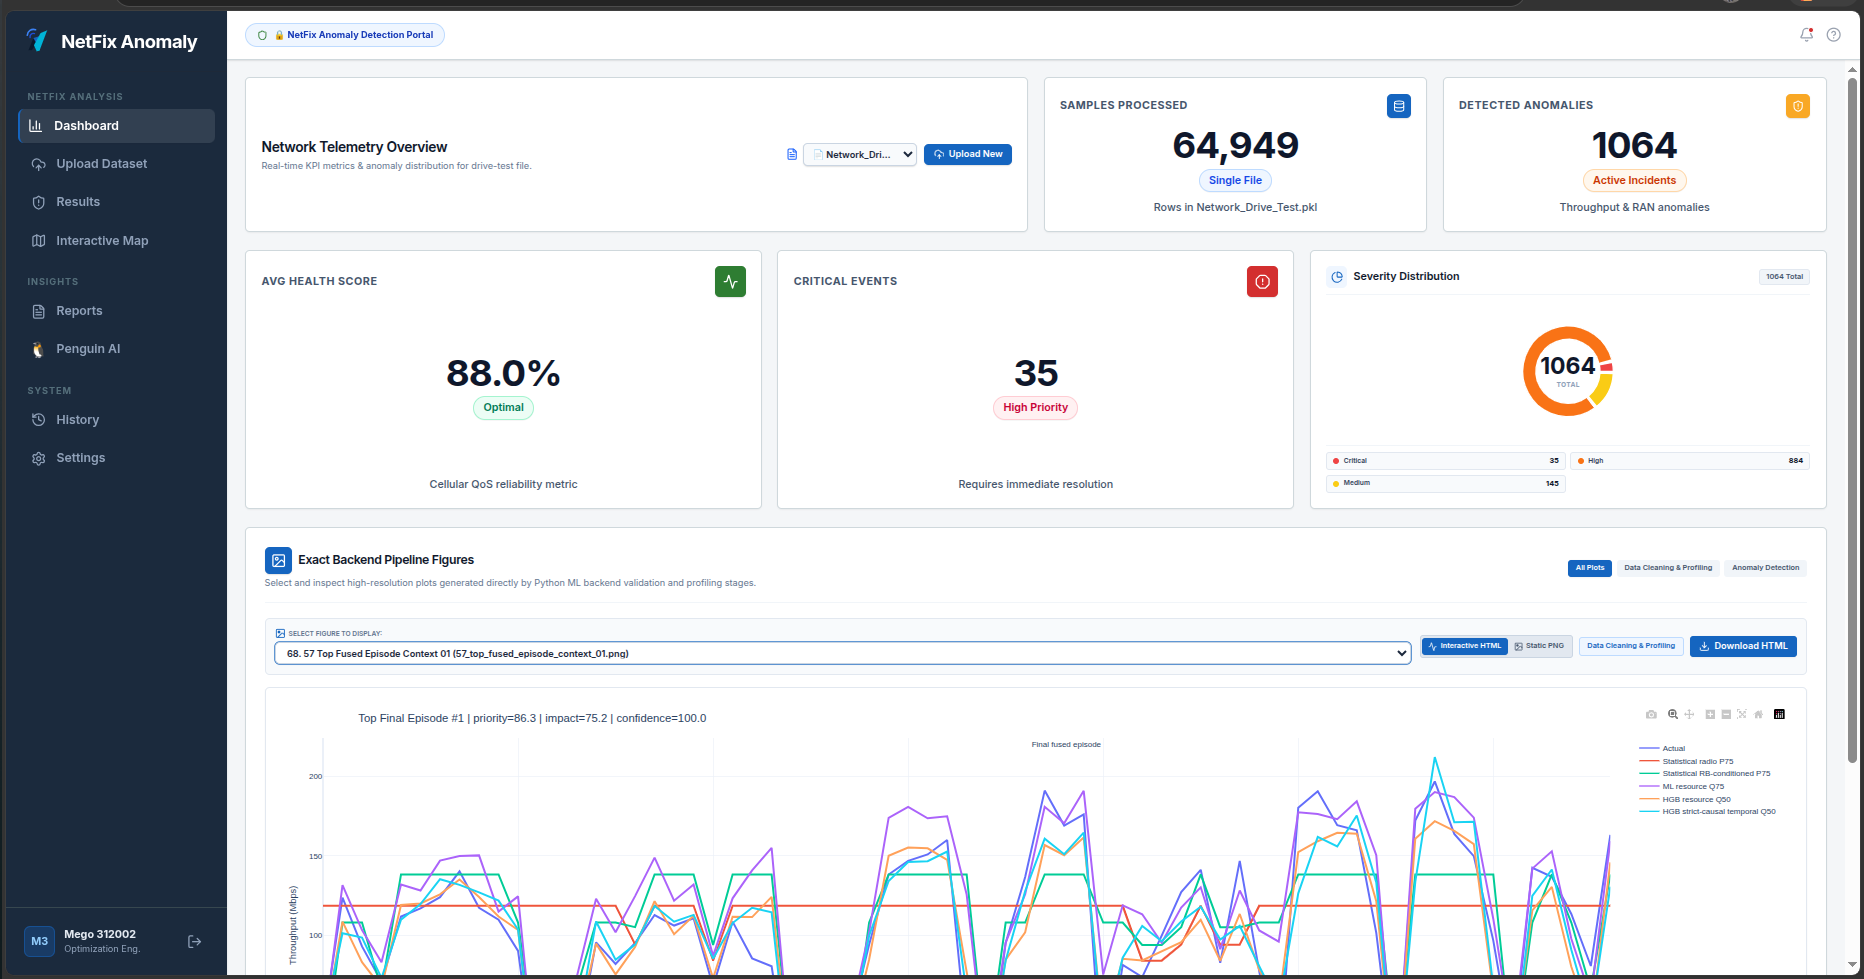
\includegraphics[width=0.95\textwidth]{images/Screenshot from 2026-08-12 14-38-38.png}
\caption{NetFix Anomaly Dashboard displaying live telemetry metrics, 1,064 detected incidents, severity donut distribution, and interactive backend pipeline time-series figures.}
\label{fig:ui_dashboard}
\end{figure}

\subsubsection{Top Telemetry Metric Cards}
\begin{table}[htbp]
\centering
\caption{Dashboard Telemetry Overview Metric Specifications.}
\label{tab:dash_metrics}
\small
\begin{tabular}{llp{7.5cm}}
\toprule
\textbf{Metric Card Title} & \textbf{Observed Value} & \textbf{Technical Description \& Scope} \\
\midrule
\textbf{SAMPLES PROCESSED} & \textbf{64,949} & Total telemetry measurement rows loaded from \texttt{Network\_Drive\_Test.pkl}. Marked with \texttt{Single File} badge. \\
\textbf{DETECTED ANOMALIES} & \textbf{1,064} & Total active incident episodes detected across throughput and radio parameters. Marked with \texttt{Active Incidents} badge. \\
\textbf{AVG HEALTH SCORE} & \textbf{88.0\%} & Cellular Quality of Service (QoS) reliability score. Marked with green \texttt{Optimal} health status badge. \\
\textbf{CRITICAL EVENTS} & \textbf{35} & High-priority operational anomalies requiring immediate engineering resolution. Marked with red alert icon. \\
\bottomrule
\end{tabular}
\end{table}

\subsubsection{Severity Distribution Analytics}
The dashboard features an interactive donut chart breaking down the 1,064 detected incidents by operational severity:
\begin{itemize}
    \item \textbf{Critical (Red):} 35 incidents ($3.3\%$). Severe throughput drop or radio link failure.
    \item \textbf{High (Orange):} 884 incidents ($83.1\%$). Significant throughput degradation below statistical P75.
    \item \textbf{Medium (Yellow):} 145 incidents ($13.6\%$). Moderate KPI variance or localized cell-edge drops.
\end{itemize}

\subsubsection{Exact Backend Pipeline Figures Panel}
Allows engineers to inspect high-resolution validation figures generated by the Python ML backend:
\begin{itemize}
    \item \textbf{Figure Selection Dropdown:} Allows selecting generated artifacts (e.g., \texttt{68. 57 Top Fused Episode Context 01 (57\_top\_fused\_episode\_context\_01.png)}).
    \item \textbf{View Mode Triggers:} Toggle between \textbf{Interactive HTML}, \textbf{Static PNG}, \textbf{Data Cleaning \& Profiling}, and \textbf{Download HTML}.
    \item \textbf{Plot Axis \& Legend Breakdown:} Plots Throughput ($0$--$200$ Mbps) against sequence index:
    \begin{itemize}
        \item \texttt{Actual Throughput} (Solid cyan line): Live recorded mobile payload speed.
        \item \texttt{Statistical radio P75} (Red baseline): 75th percentile expected throughput based on cell radio state.
        \item \texttt{Statistical RB-conditioned P75} (Orange baseline): Resource-block conditioned expected throughput.
        \item \texttt{ML resource Q75} (Purple curve): 75th percentile quantile regression from ML feature space.
        \item \texttt{HGB resource Q50} (Yellow curve): Histogram Gradient Boosting median resource expectation.
        \item \texttt{HGB strict-causal temporal Q50} (Blue curve): Strict-causal temporal sequence prediction.
    \end{itemize}
\end{itemize}

---

\subsection{Module 2: Dataset Ingestion \& 4-Stage Stepper}
\textit{Reference Screenshot: \texttt{Screenshot from 2026-08-12 14-38-48.png}}

The \textbf{Upload Dataset} page orchestrates file ingestion and real-time execution feedback.

\begin{figure}[htbp]
\centering
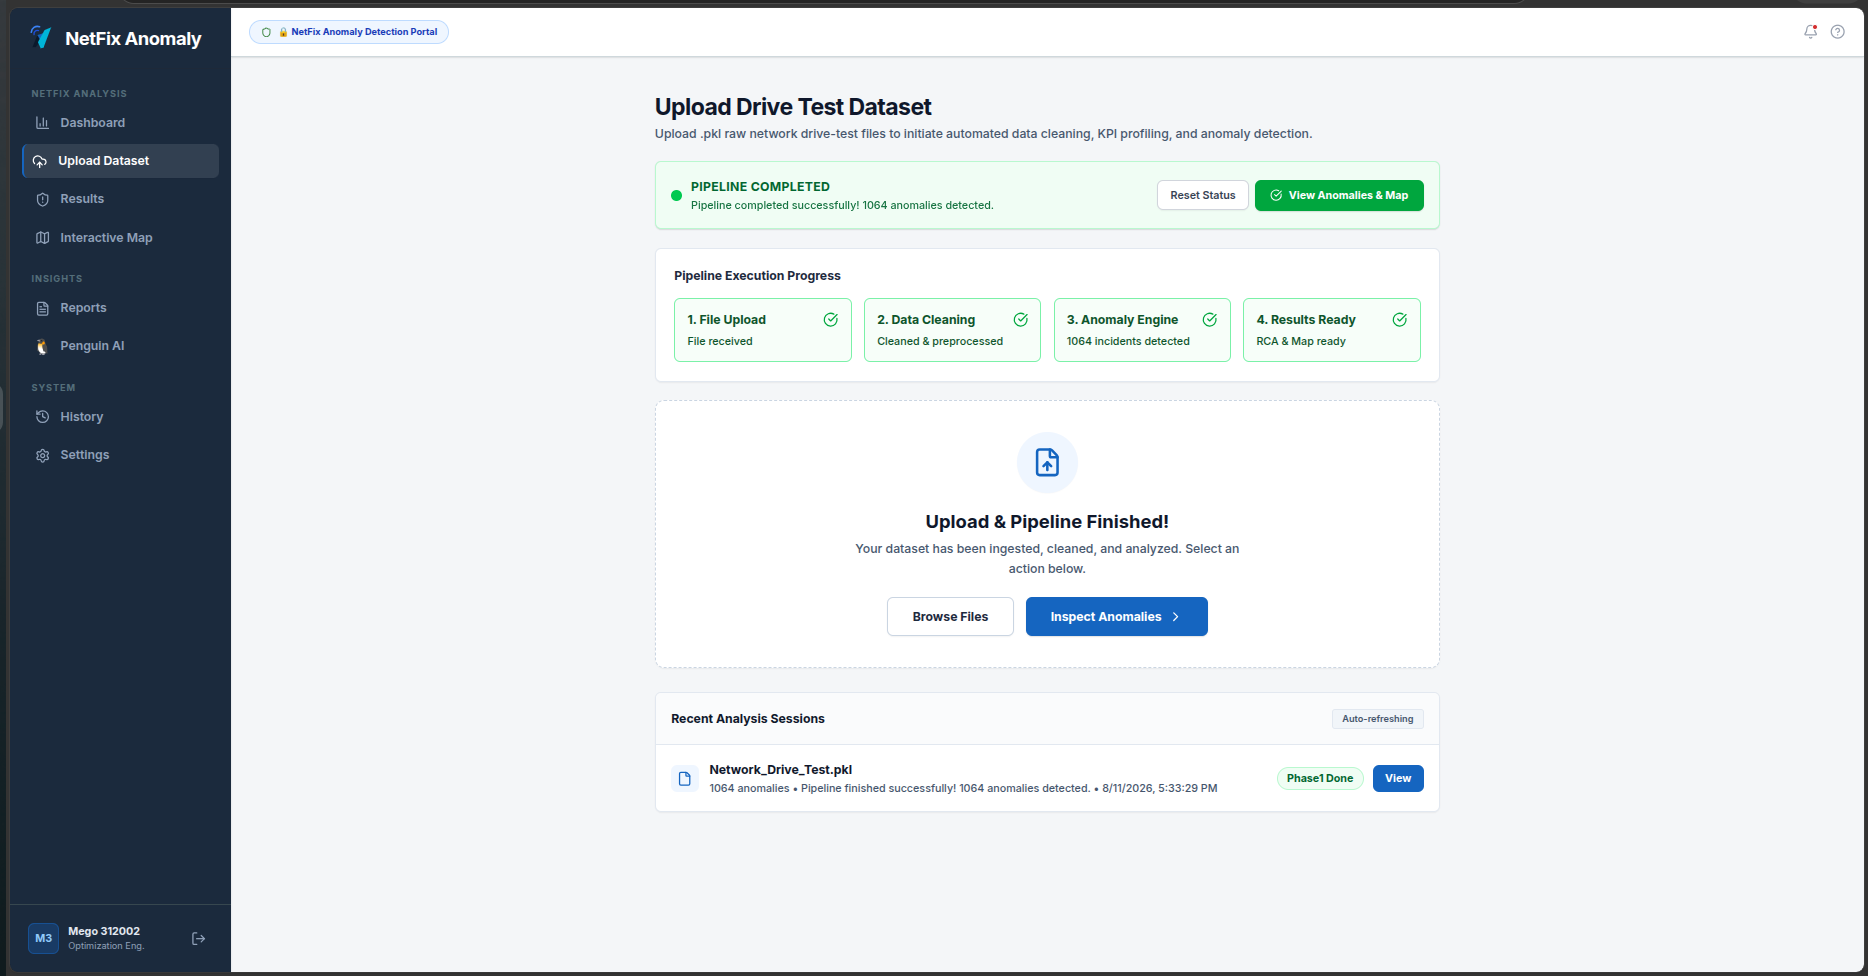
\includegraphics[width=0.95\textwidth]{images/Screenshot from 2026-08-12 14-38-48.png}
\caption{Upload Dataset page showing 4-stage execution stepper (File Upload, Data Cleaning, Anomaly Engine, Results Ready) and recent session audit log.}
\label{fig:ui_upload}
\end{figure}

\subsubsection{4-Stage Execution Progress Stepper}
\begin{enumerate}
    \item \textbf{1. File Upload (Completed $\checkmark$):} Validates file payload integrity and receives raw \texttt{.pkl} network drive-test file.
    \item \textbf{2. Data Cleaning (Completed $\checkmark$):} Executes 11-stage non-leaking preprocessing pipeline (\texttt{ran-cleaning-service}).
    \item \textbf{3. Anomaly Engine (Completed $\checkmark$):} Runs 19-stage statistical, HGB ML, and PyTorch LSTM anomaly fusion models (\textbf{1,064 incidents detected}).
    \item \textbf{4. Results Ready (Completed $\checkmark$):} Constructs MongoDB session indexes and prepares RCA cause-matching and GIS map artifacts.
\end{enumerate}

\subsubsection{Pipeline Completed Banner \& Controls}
Upon completion, a green status banner displays:
\begin{center}
\texttt{PIPELINE COMPLETED ── Pipeline completed successfully! 1064 anomalies detected.}
\end{center}
Engineers can click \textbf{View Anomalies \& Map} to jump directly to the GIS map or \textbf{Reset Status} to prepare for a new file upload.

\subsubsection{Recent Analysis Sessions Audit Log}
Displays active sessions in a clean tabular view containing Dataset Name (\texttt{Network\_Drive\_Test.pkl}), Anomaly Count (\texttt{1064 anomalies}), Timestamp (\texttt{8/11/2026, 5:33:29 PM}), Pipeline Status Badge (\texttt{Phase1 Done}), and a direct \textbf{View} session button.

---

\subsection{Module 3: Deterministic RCA Engine \& Telemetry Evidence}
\textit{Reference Screenshots: \texttt{Screenshot from 2026-08-12 14-39-04.png} \& \texttt{14-39-08.png}}

The \textbf{Results} view provides deep-dive root cause analysis for individual anomaly incidents.

\begin{figure}[htbp]
\centering
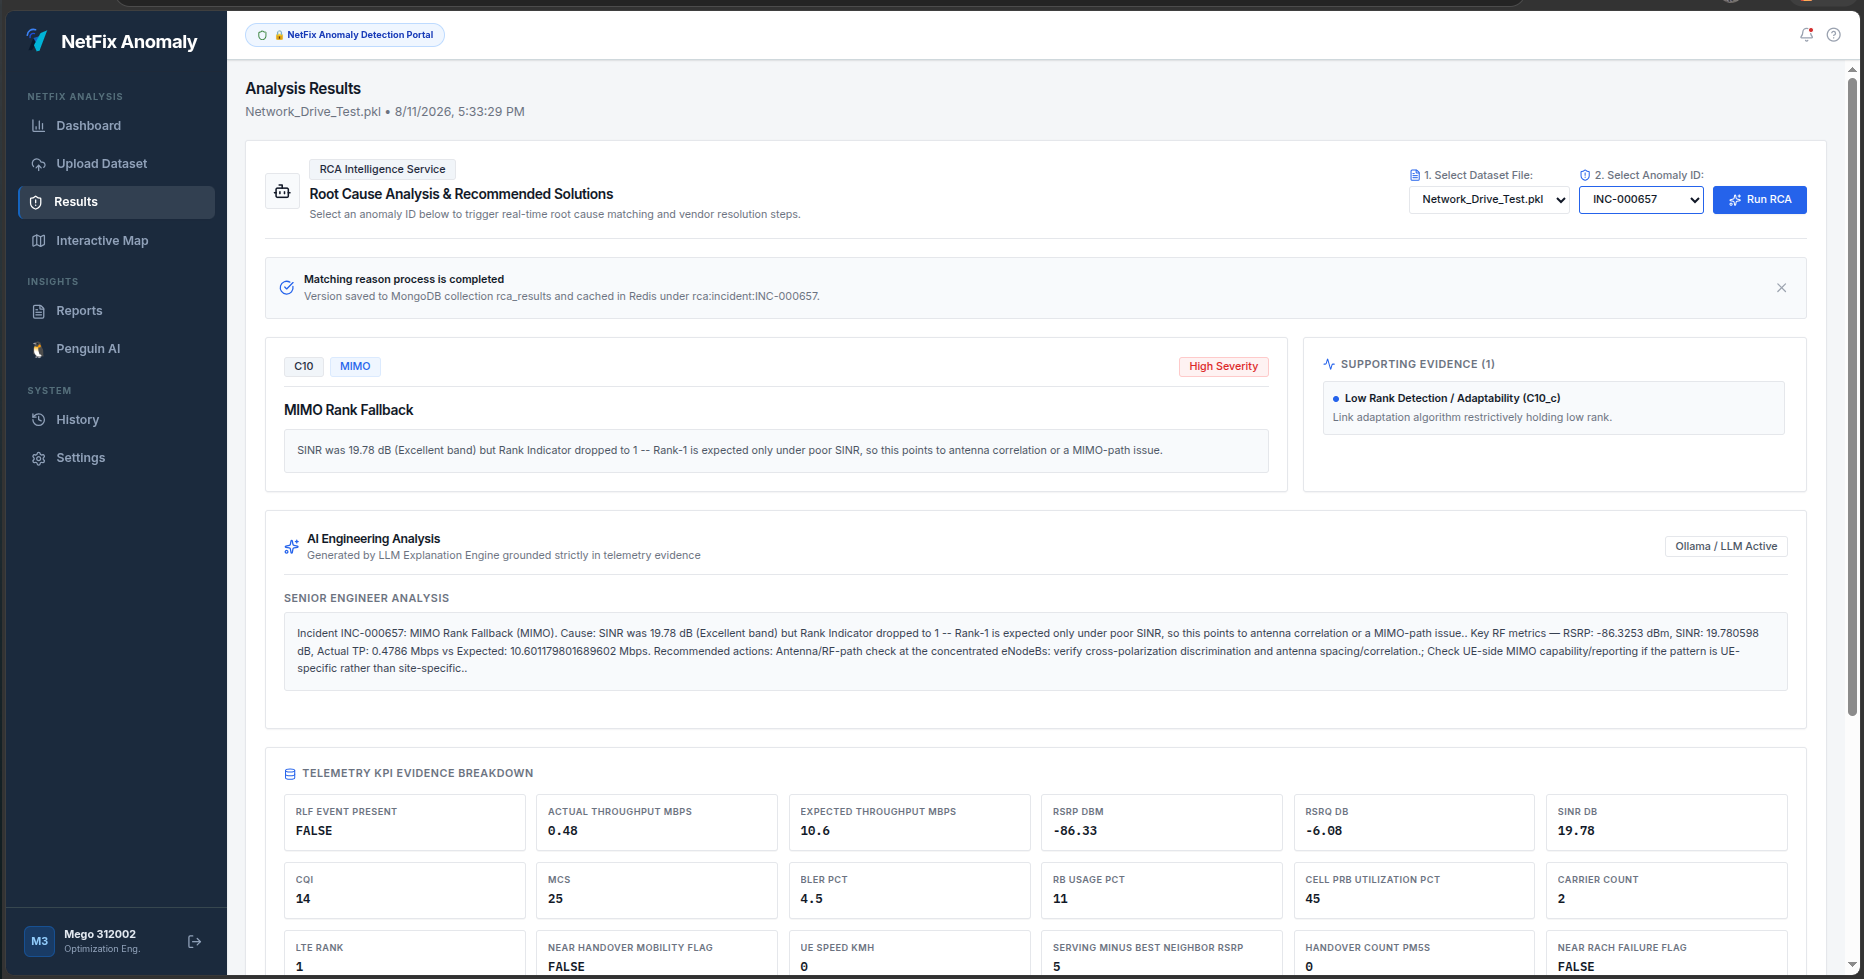
\includegraphics[width=0.95\textwidth]{images/Screenshot from 2026-08-12 14-39-04.png}
\caption{Results page displaying matched rule card (C10 MIMO Rank Fallback), Ollama AI Senior Engineer analysis, and 23-metric telemetry evidence breakdown grid.}
\label{fig:ui_rca_grid}
\end{figure}

\begin{figure}[htbp]
\centering
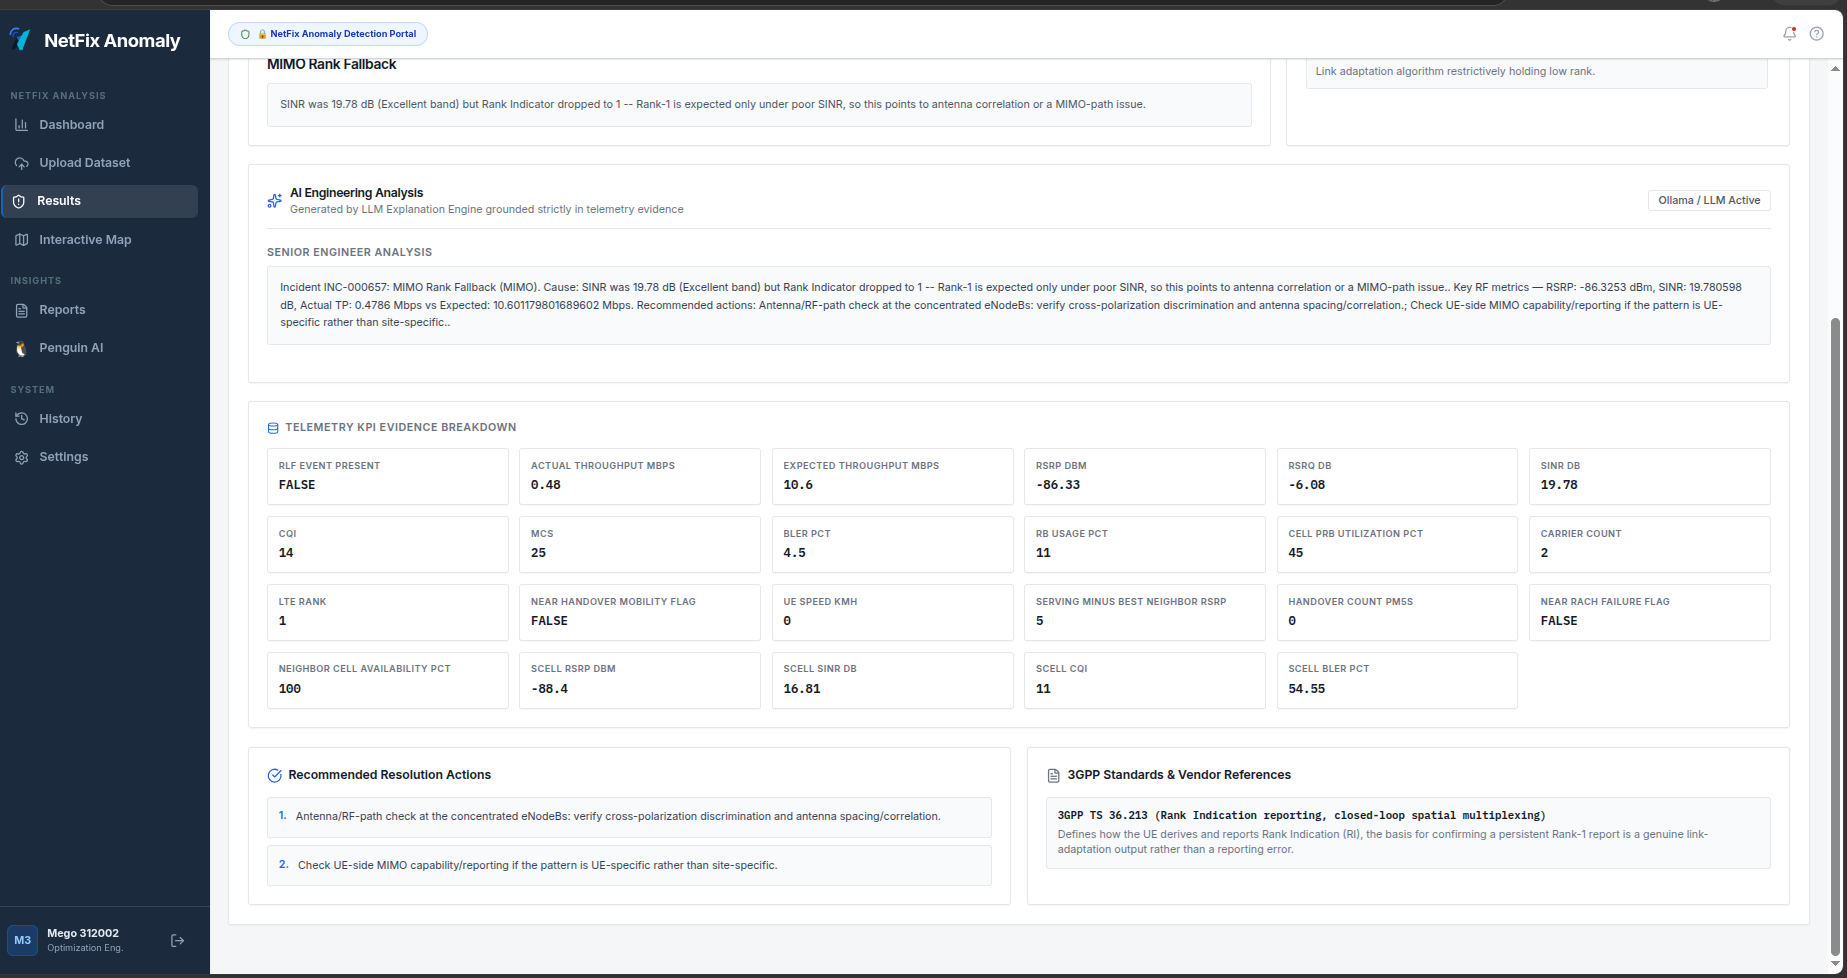
\includegraphics[width=0.95\textwidth]{images/Screenshot from 2026-08-12 14-39-08.png}
\caption{Results page displaying recommended resolution actions and official 3GPP TS 36.213 standards reference.}
\label{fig:ui_rca_recs}
\end{figure}

\subsubsection{Incident Selection Header}
Engineers select the target dataset (\texttt{Network\_Drive\_Test.pkl}) and target Incident ID (e.g., \texttt{INC-000657}) via drop-down selectors, then click \textbf{Run RCA}. A status confirmation banner verifies:
\begin{center}
\small\texttt{Matching reason process is completed ── Version saved to MongoDB collection rca\_results and cached in Redis under rca:incident:INC-000657.}
\end{center}

\subsubsection{Rule-Based Match Card (e.g., Incident INC-000657)}
\begin{itemize}
    \item \textbf{Category \& Badges:} \texttt{C10}, \texttt{MIMO}, \texttt{High Severity}.
    \item \textbf{Matched Reason Title:} \textbf{MIMO Rank Fallback}
    \item \textbf{Cause Narrative:} \textit{``SINR was 19.78 dB (Excellent band) but Rank Indicator dropped to 1 -- Rank-1 is expected only under poor SINR, so this points to antenna correlation or a MIMO-path issue.''}
    \item \textbf{Supporting Evidence Panel:} \texttt{Low Rank Detection / Adaptability (C10\_c)}: Link adaptation algorithm restrictively holding low rank despite clean RF conditions.
\end{itemize}

\subsubsection{AI Engineering Analysis Card (Local Ollama Engine)}
Synthesizes grounded commentary combining ML metrics and physical layer phenomena:
\begin{quote}
\small
\textbf{SENIOR ENGINEER ANALYSIS:} Incident INC-000657: MIMO Rank Fallback (MIMO). Cause: SINR was 19.78 dB (Excellent band) but Rank Indicator dropped to 1 -- Rank-1 is expected only under poor SINR, so this points to antenna correlation or a MIMO-path issue. Key RF metrics — RSRP: -86.3253 dBm, SINR: 19.780598 dB, Actual TP: 0.4786 Mbps vs Expected: 10.601179 Mbps. Recommended actions: Antenna/RF-path check at the concentrated eNodeBs: verify cross-polarization discrimination and antenna spacing/correlation; Check UE-side MIMO capability/reporting if the pattern is UE-specific rather than site-specific.
\end{quote}

\subsubsection{23-Metric Telemetry Evidence Breakdown Grid}
Presents a complete 23-card telemetry metric grid extracted from MongoDB for the exact anomaly timestamp:
\begin{table}[htbp]
\centering
\caption{Incident INC-000657 Telemetry Evidence Grid Breakdown.}
\label{tab:inc_657_grid}
\small
\begin{tabular}{lll}
\toprule
\textbf{Telemetry Metric Field} & \textbf{Recorded Value} & \textbf{Evaluation \& State} \\
\midrule
\texttt{RLF EVENT PRESENT} & \textbf{FALSE} & No Radio Link Failure event. \\
\texttt{ACTUAL THROUGHPUT MBPS} & \textbf{0.48 Mbps} & Severe degradation (Expected: 10.6 Mbps). \\
\texttt{EXPECTED THROUGHPUT MBPS} & \textbf{10.6 Mbps} & Calculated P75 baseline for cell. \\
\texttt{RSRP DBM} & \textbf{-86.33 dBm} & Good serving cell signal strength. \\
\texttt{RSRQ DB} & \textbf{-6.08 dB} & Good serving cell signal quality. \\
\texttt{SINR DB} & \textbf{19.78 dB} & Excellent Signal-to-Interference Ratio. \\
\texttt{CQI} & \textbf{14} & High Channel Quality Indicator (64QAM/256QAM). \\
\texttt{MCS} & \textbf{25} & High Modulation \& Coding Scheme index. \\
\texttt{BLER PCT} & \textbf{4.5\%} & Low Block Error Rate ($<5\%$). \\
\texttt{RB USAGE PCT} & \textbf{11\%} & Low Resource Block usage. \\
\texttt{CELL PRB UTILIZATION PCT} & \textbf{45\%} & Moderate Cell load. \\
\texttt{CARRIER COUNT} & \textbf{2} & Dual Component Carrier (CA active). \\
\texttt{LTE RANK} & \textbf{1} & \textbf{ANOMALOUS (Rank 1 under 19.78 dB SINR)}. \\
\texttt{NEAR HANDOVER MOBILITY FLAG} & \textbf{FALSE} & Stationary / Low mobility state. \\
\texttt{UE SPEED KMH} & \textbf{0 km/h} & Stationary User Equipment. \\
\texttt{SERVING MINUS BEST NEIGHBOR RSRP} & \textbf{5 dB} & Adequate cell dominance margin. \\
\texttt{HANDOVER COUNT PM5S} & \textbf{0} & No recent handovers. \\
\texttt{NEAR RACH FAILURE FLAG} & \textbf{FALSE} & Random Access Channel normal. \\
\texttt{NEIGHBOR CELL AVAILABILITY PCT} & \textbf{100\%} & All neighbor cells available. \\
\texttt{SCELL RSRP DBM} & \textbf{-88.4 dBm} & Secondary Cell RSRP clean. \\
\texttt{SCELL SINR DB} & \textbf{16.81 dB} & Secondary Cell SINR clean. \\
\texttt{SCELL CQI} & \textbf{11} & Secondary Cell CQI acceptable. \\
\texttt{SCELL BLER PCT} & \textbf{54.55\%} & Secondary Cell BLER elevated. \\
\bottomrule
\end{tabular}
\end{table}

\subsubsection{Recommended Actions \& 3GPP Standard References}
\begin{enumerate}
    \item \textbf{Action 1:} Antenna/RF-path check at concentrated eNodeBs: verify cross-polarization discrimination and antenna spacing/correlation.
    \item \textbf{Action 2:} Check UE-side MIMO capability/reporting if the pattern is UE-specific rather than site-specific.
    \item \textbf{3GPP Standard Reference:} \textbf{3GPP TS 36.213 (Rank Indication reporting, closed-loop spatial multiplexing)}: Defines how the UE derives and reports Rank Indication (RI), the basis for confirming a persistent Rank-1 report is a genuine link-adaptation output rather than a reporting error.
\end{enumerate}

---

\subsection{Module 4: Interactive GIS Trajectory Map}
\textit{Reference Screenshot: \texttt{Screenshot from 2026-08-12 14-39-17.png}}

The \textbf{Interactive Map} view renders geospatial drive-test trajectories over an interactive Leaflet canvas.

\begin{figure}[htbp]
\centering
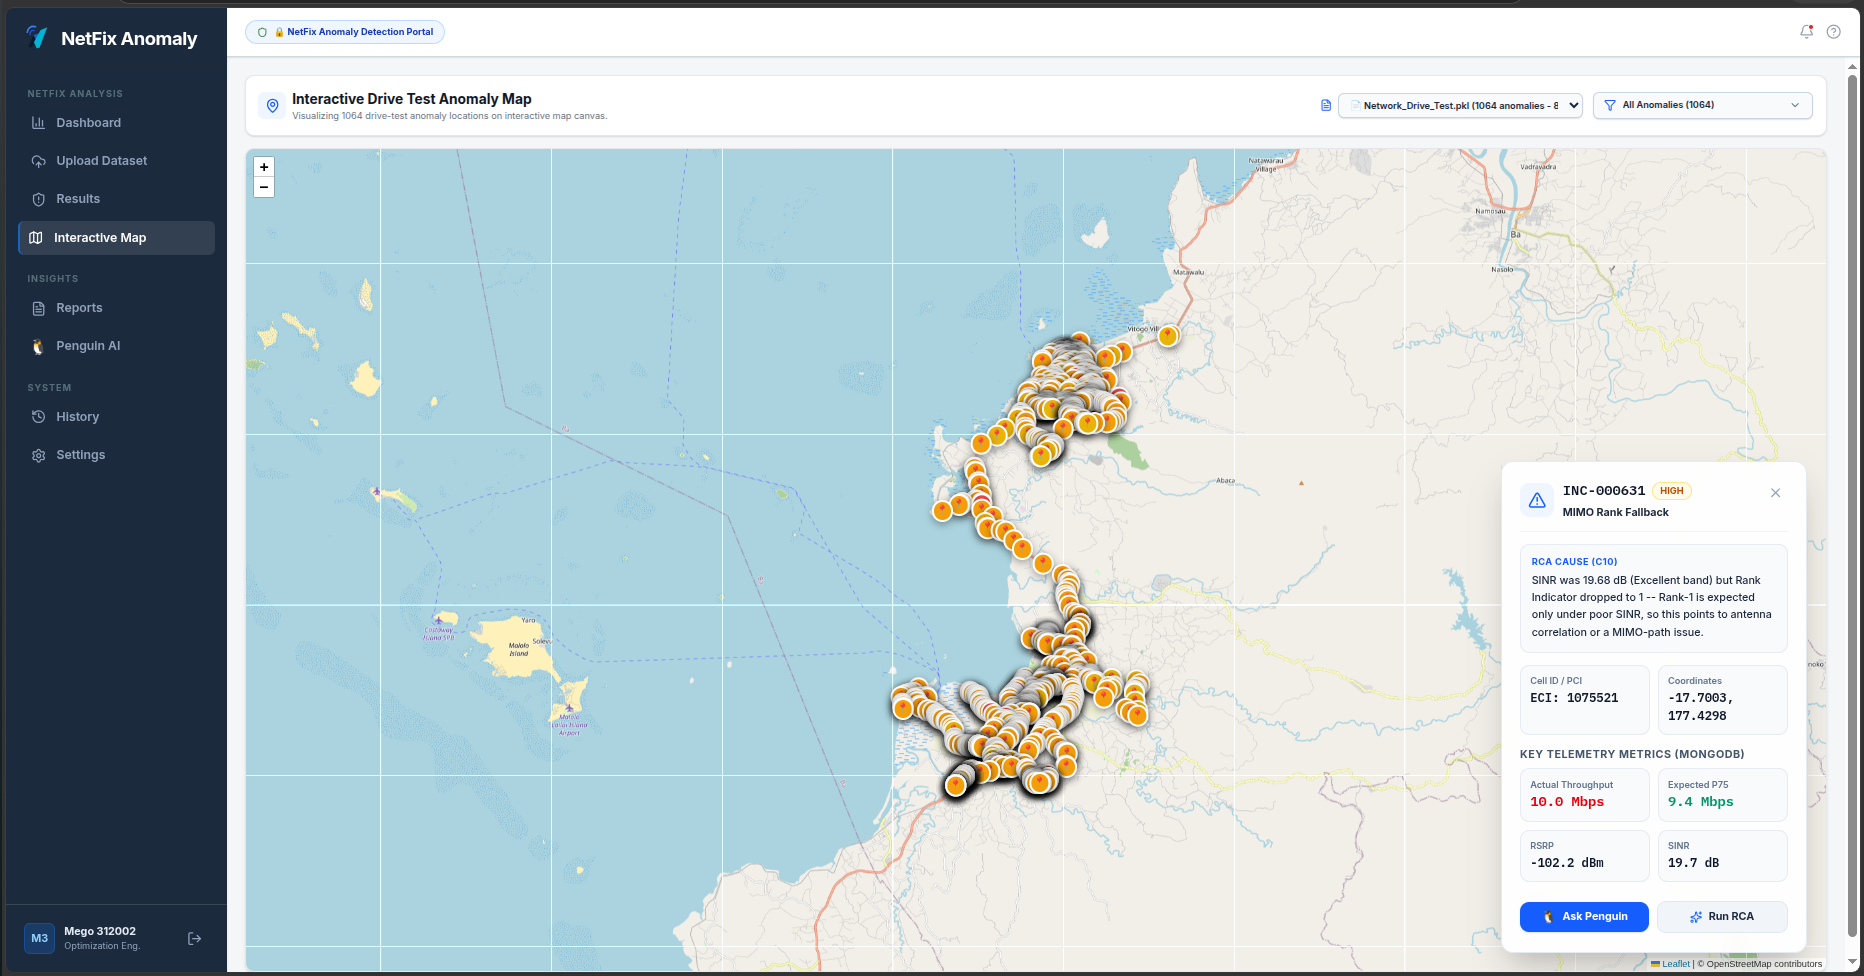
\includegraphics[width=0.95\textwidth]{images/Screenshot from 2026-08-12 14-39-17.png}
\caption{Interactive Map view showing GPS drive-test breadcrumb path, anomaly pin markers, and interactive popup for Incident INC-000631.}
\label{fig:ui_map}
\end{figure}

\subsubsection{Map Controls \& Layer Filters}
\begin{itemize}
    \item \textbf{Dataset Selector:} Switch active dataset file (\texttt{Network\_Drive\_Test.pkl}).
    \item \textbf{Incident Filter Dropdown:} Filter displayed markers (\texttt{All Anomalies (1064)} or specific severity tiers).
    \item \textbf{Zoom \& Canvas Navigation:} Full pan/zoom capabilities with custom OpenStreetMap tile rendering.
\end{itemize}

\subsubsection{Drive-Test Trajectory \& Pinplot Inspection}
The drive path is rendered as a continuous GPS breadcrumb line along coastal highway routes. Anomaly locations are highlighted with orange/white numbered pin markers. Clicking any marker (e.g., \texttt{INC-000631}) opens an interactive modal:
\begin{itemize}
    \item \textbf{Header:} Incident ID \texttt{INC-000631} with \texttt{HIGH} severity badge.
    \item \textbf{Title \& Cause (C10):} MIMO Rank Fallback (SINR 19.68 dB, Rank Indicator 1).
    \item \textbf{Metadata Grid:} Cell ID / PCI (\texttt{ECI: 1075521}), GPS Coordinates (\texttt{-17.7003, 177.4298}).
    \item \textbf{Key Telemetry Metrics (MongoDB):} Actual Throughput (\textbf{10.0 Mbps}), Expected P75 (\textbf{9.4 Mbps}), RSRP (\textbf{-102.2 dBm}), SINR (\textbf{19.7 dB}).
    \item \textbf{Quick Action Buttons:} \textbf{Ask Penguin} (launches AI Assistant with pre-loaded incident context) and \textbf{Run RCA} (jumps to detailed RCA results).
\end{itemize}

---

\subsection{Module 5: Penguin AI Copilot \& Report Generator}
\textit{Reference Screenshots: \texttt{Screenshot from 2026-08-11 20-52-29.png} to \texttt{20-52-49.png}, \texttt{14-39-31.png}}

The \textbf{Penguin AI} page integrates a local conversational LLM assistant fine-tuned for telecom telemetry diagnostics.

\begin{figure}[htbp]
\centering
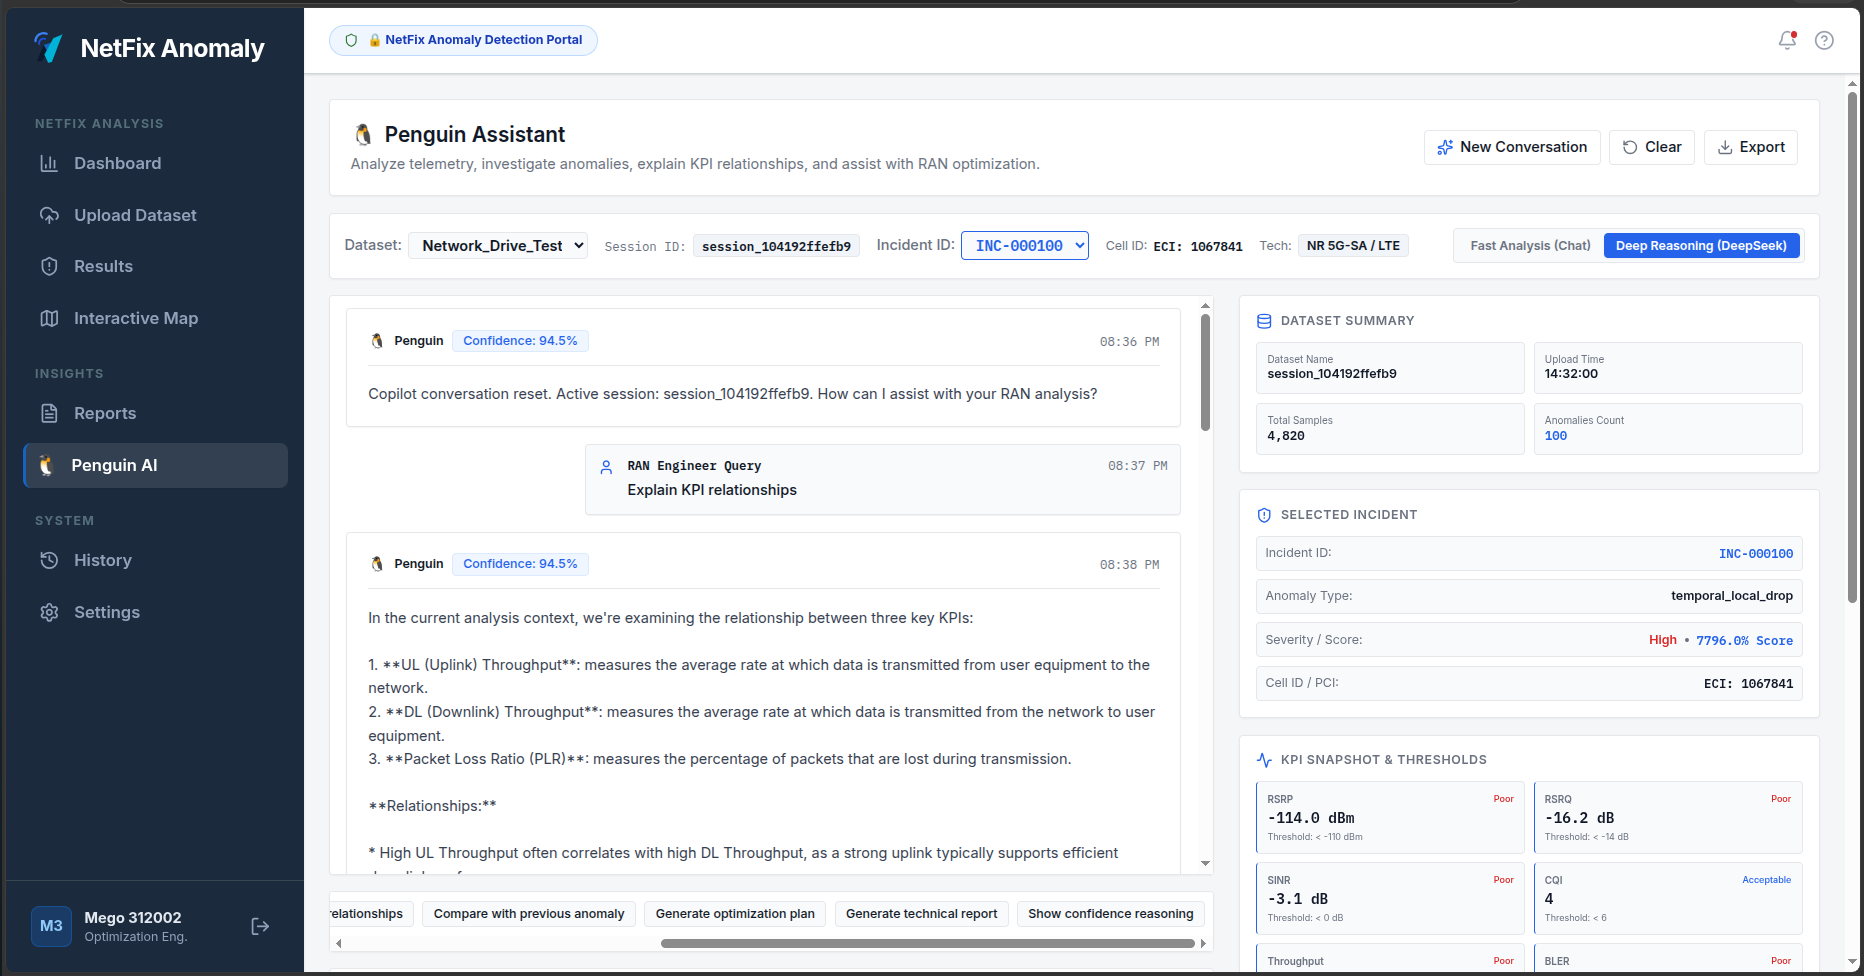
\includegraphics[width=0.95\textwidth]{images/Screenshot from 2026-08-11 20-52-29.png}
\caption{Penguin AI Assistant interface demonstrating conversational KPI relationship explanation and incident context sidebars.}
\label{fig:ui_penguin_1}
\end{figure}

\begin{figure}[htbp]
\centering
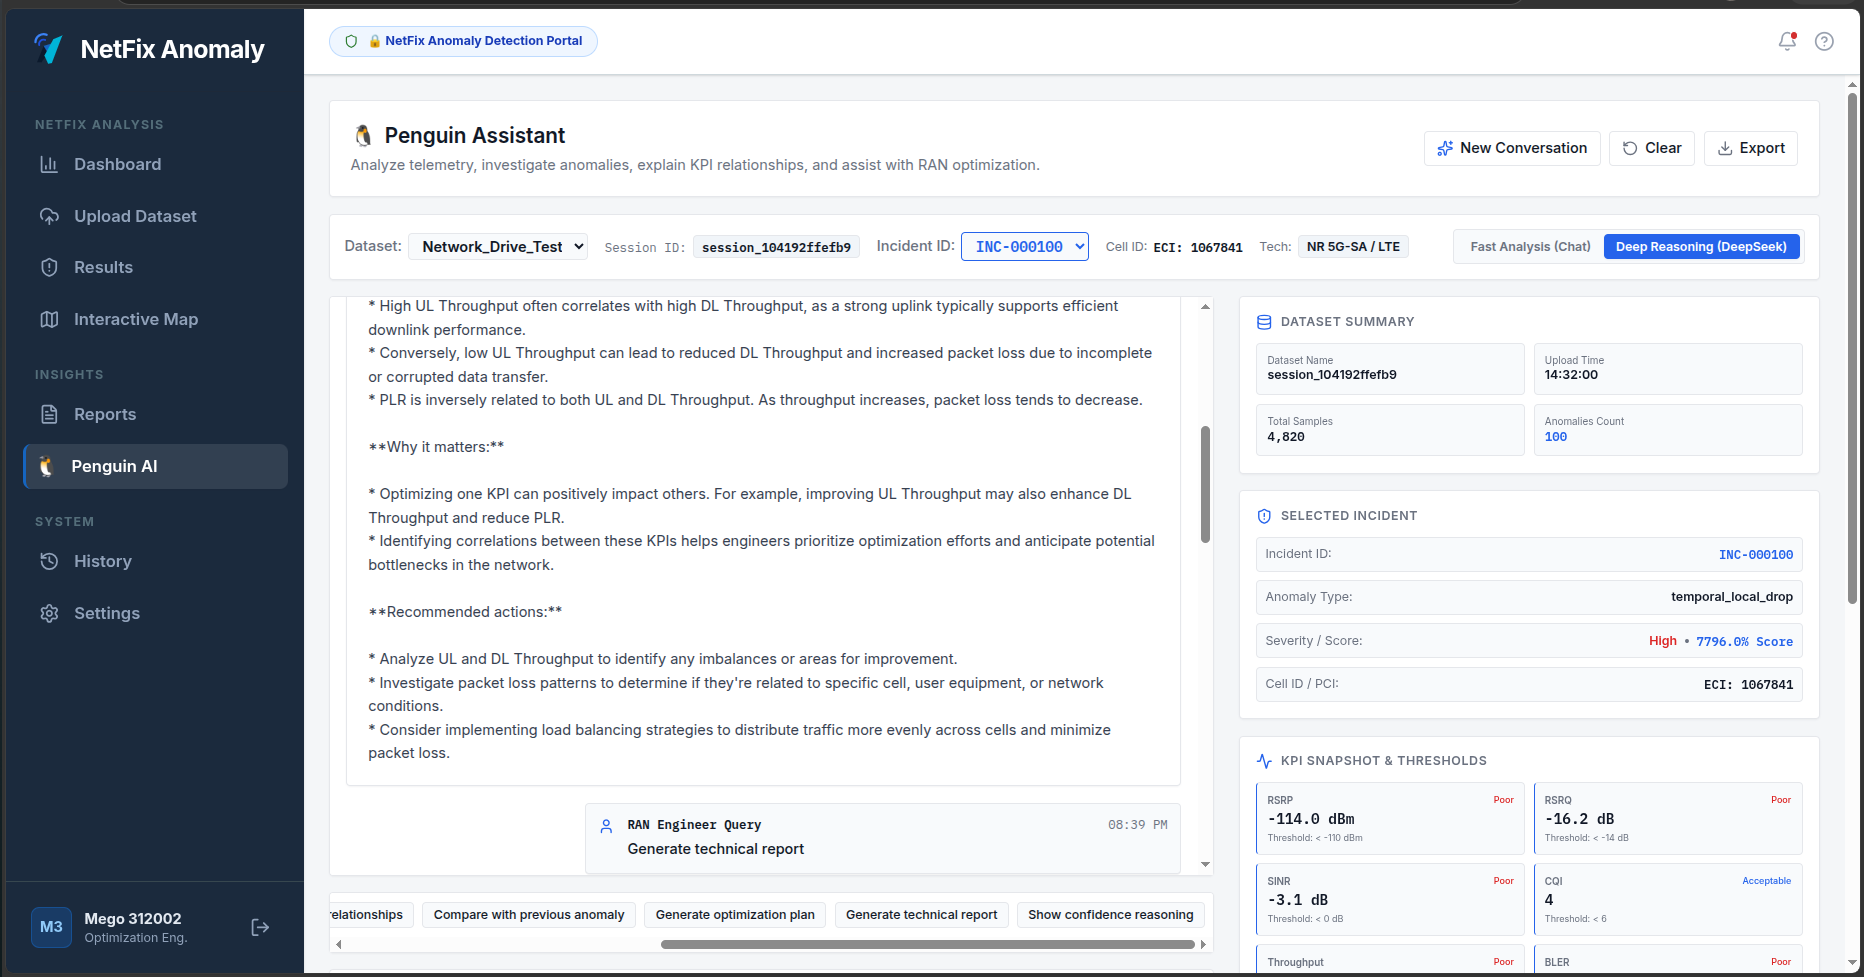
\includegraphics[width=0.95\textwidth]{images/Screenshot from 2026-08-11 20-52-37.png}
\caption{Penguin AI Assistant continuing KPI relationship analysis and offering quick action triggers.}
\label{fig:ui_penguin_2}
\end{figure}

\begin{figure}[htbp]
\centering
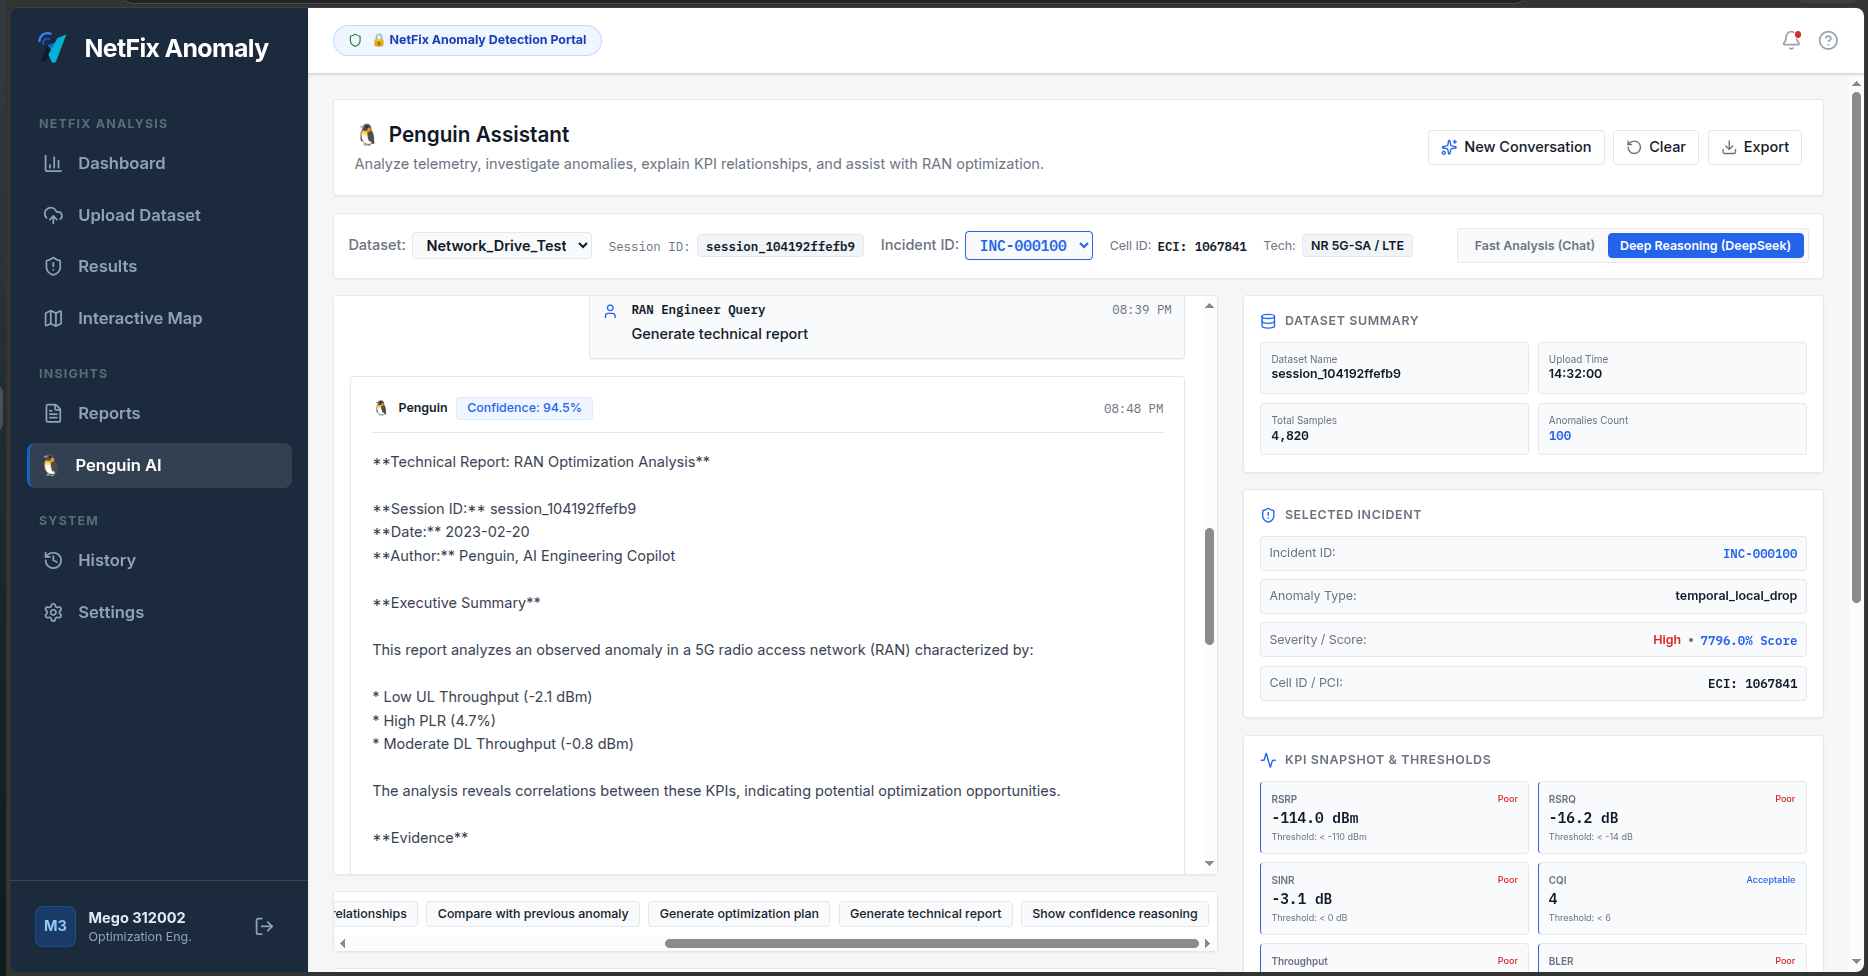
\includegraphics[width=0.95\textwidth]{images/Screenshot from 2026-08-11 20-52-42.png}
\caption{Penguin AI Assistant generating automated technical report executive summary.}
\label{fig:ui_penguin_report_1}
\end{figure}

\begin{figure}[htbp]
\centering
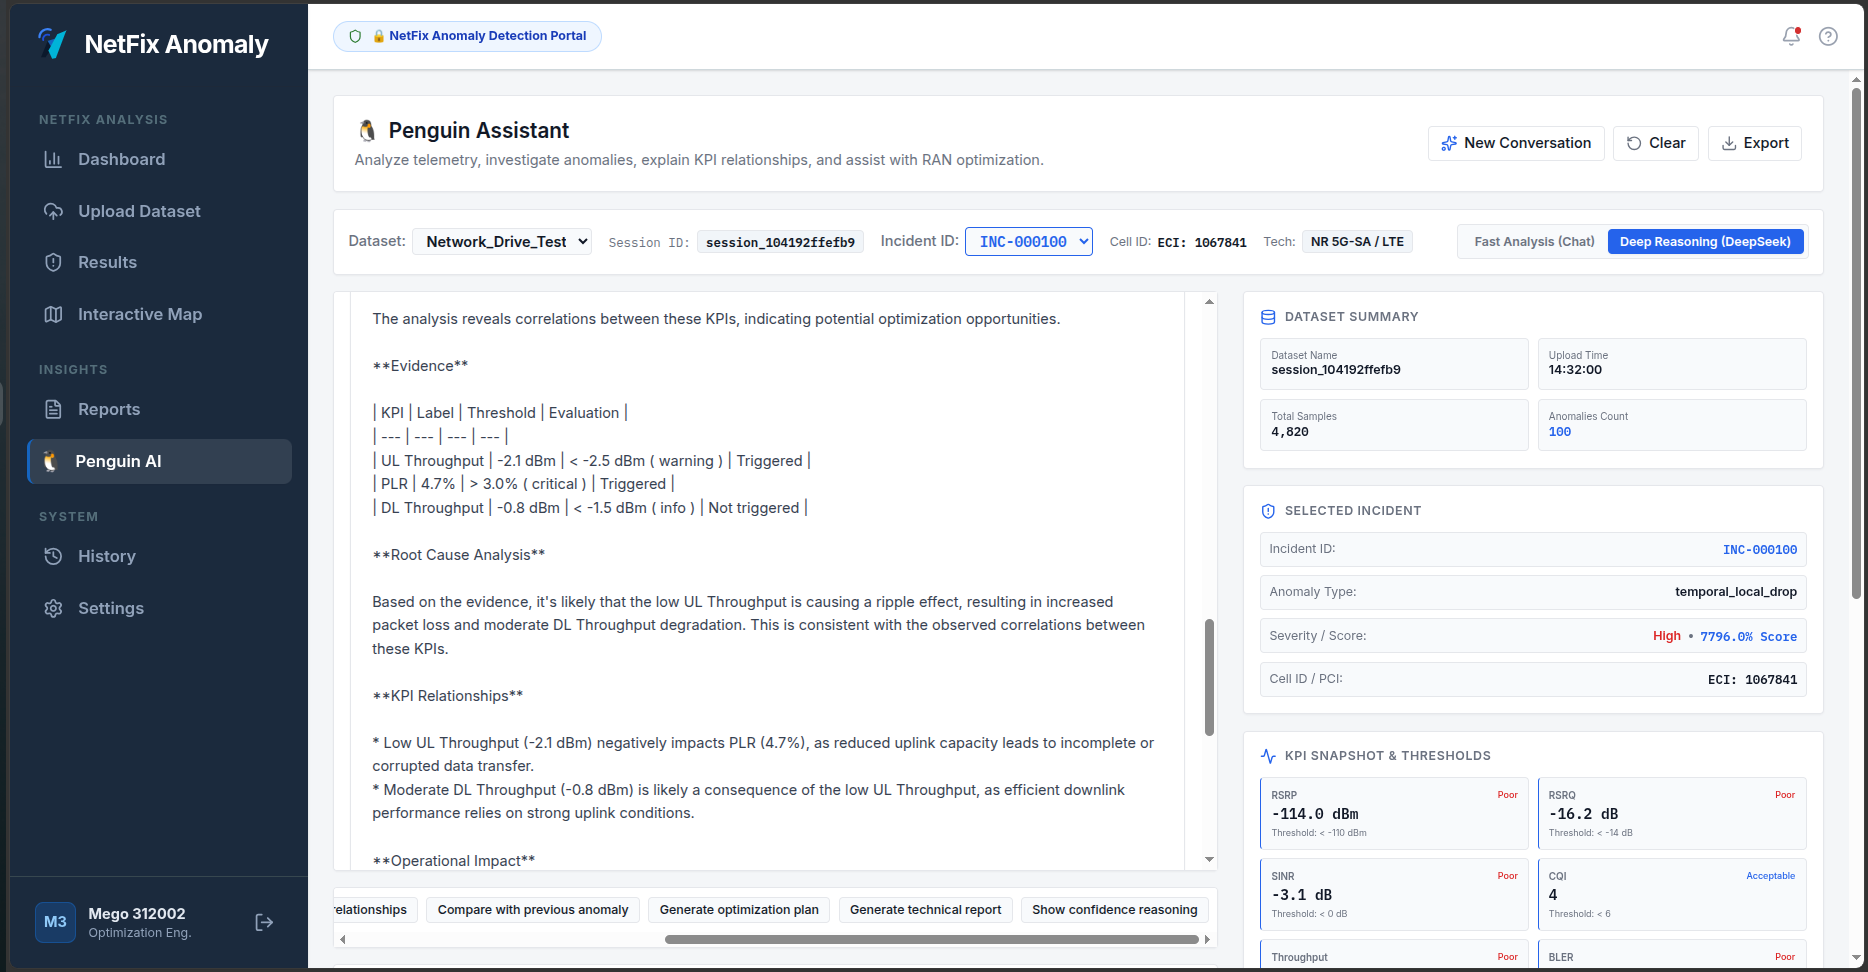
\includegraphics[width=0.95\textwidth]{images/Screenshot from 2026-08-11 20-52-46.png}
\caption{Penguin AI Assistant generating technical report evidence table and root cause diagnosis.}
\label{fig:ui_penguin_report_2}
\end{figure}

\begin{figure}[htbp]
\centering
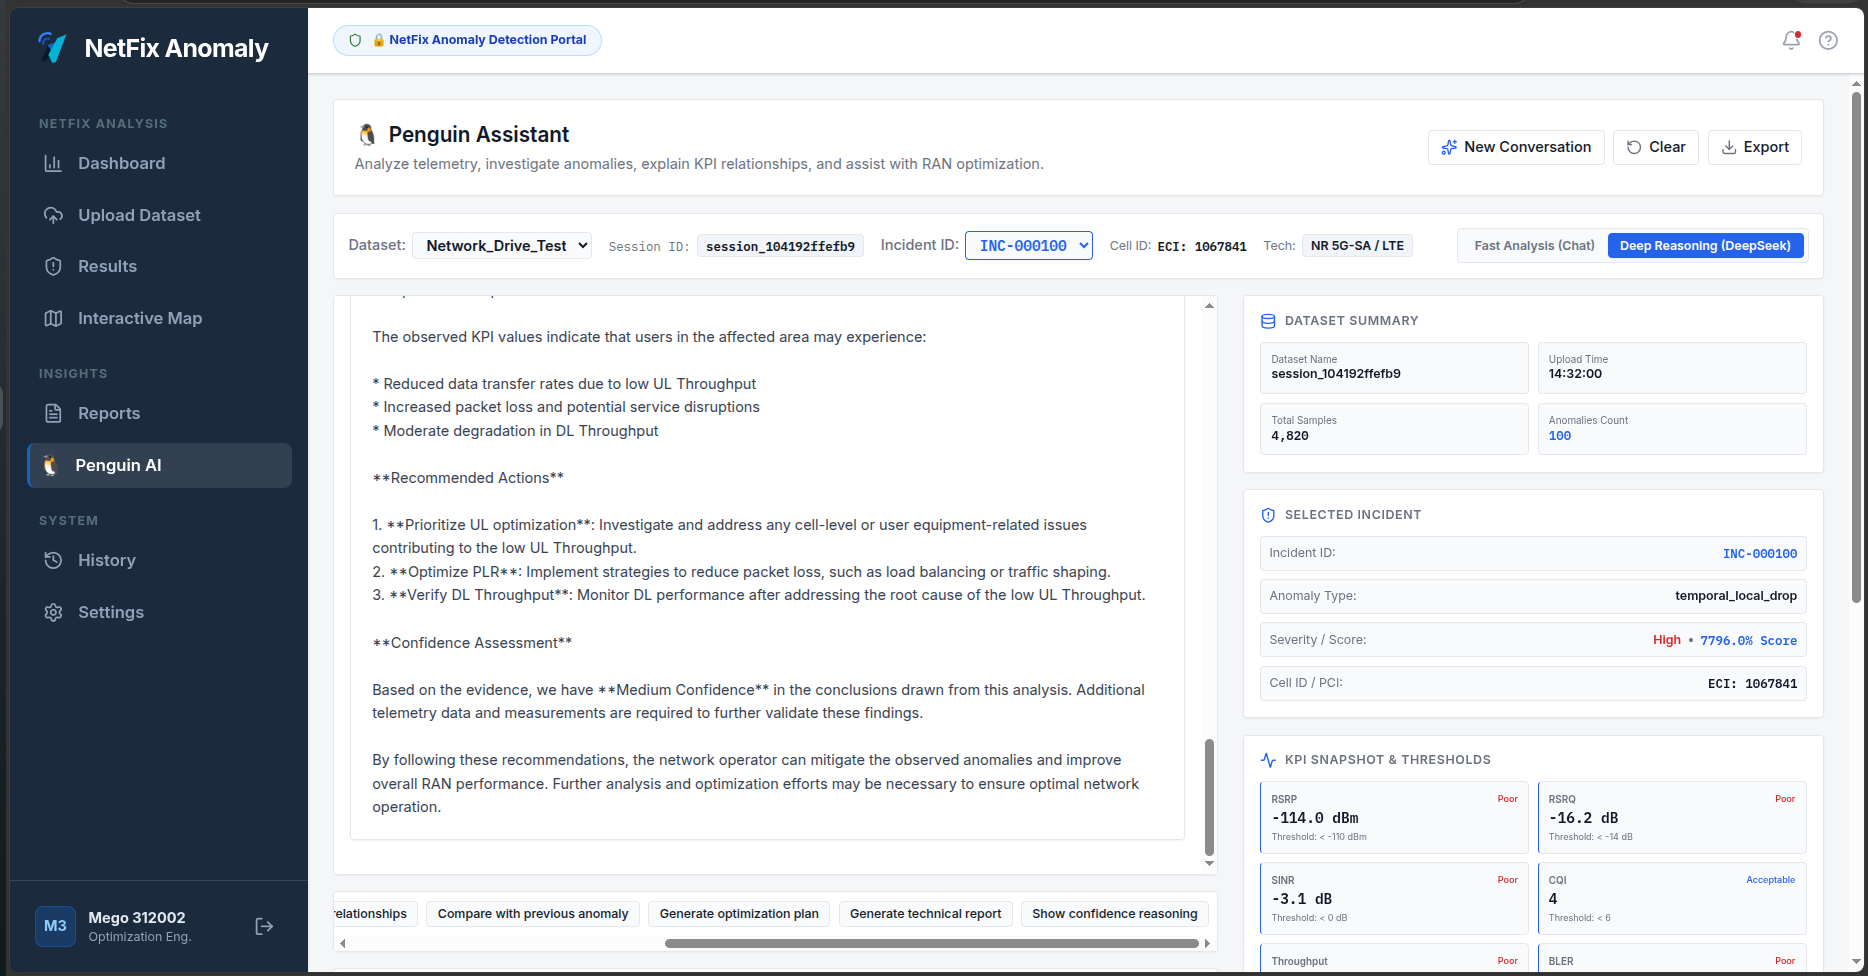
\includegraphics[width=0.95\textwidth]{images/Screenshot from 2026-08-11 20-52-49.png}
\caption{Penguin AI Assistant finalizing technical report recommended actions and confidence assessment.}
\label{fig:ui_penguin_report_3}
\end{figure}

\begin{figure}[htbp]
\centering
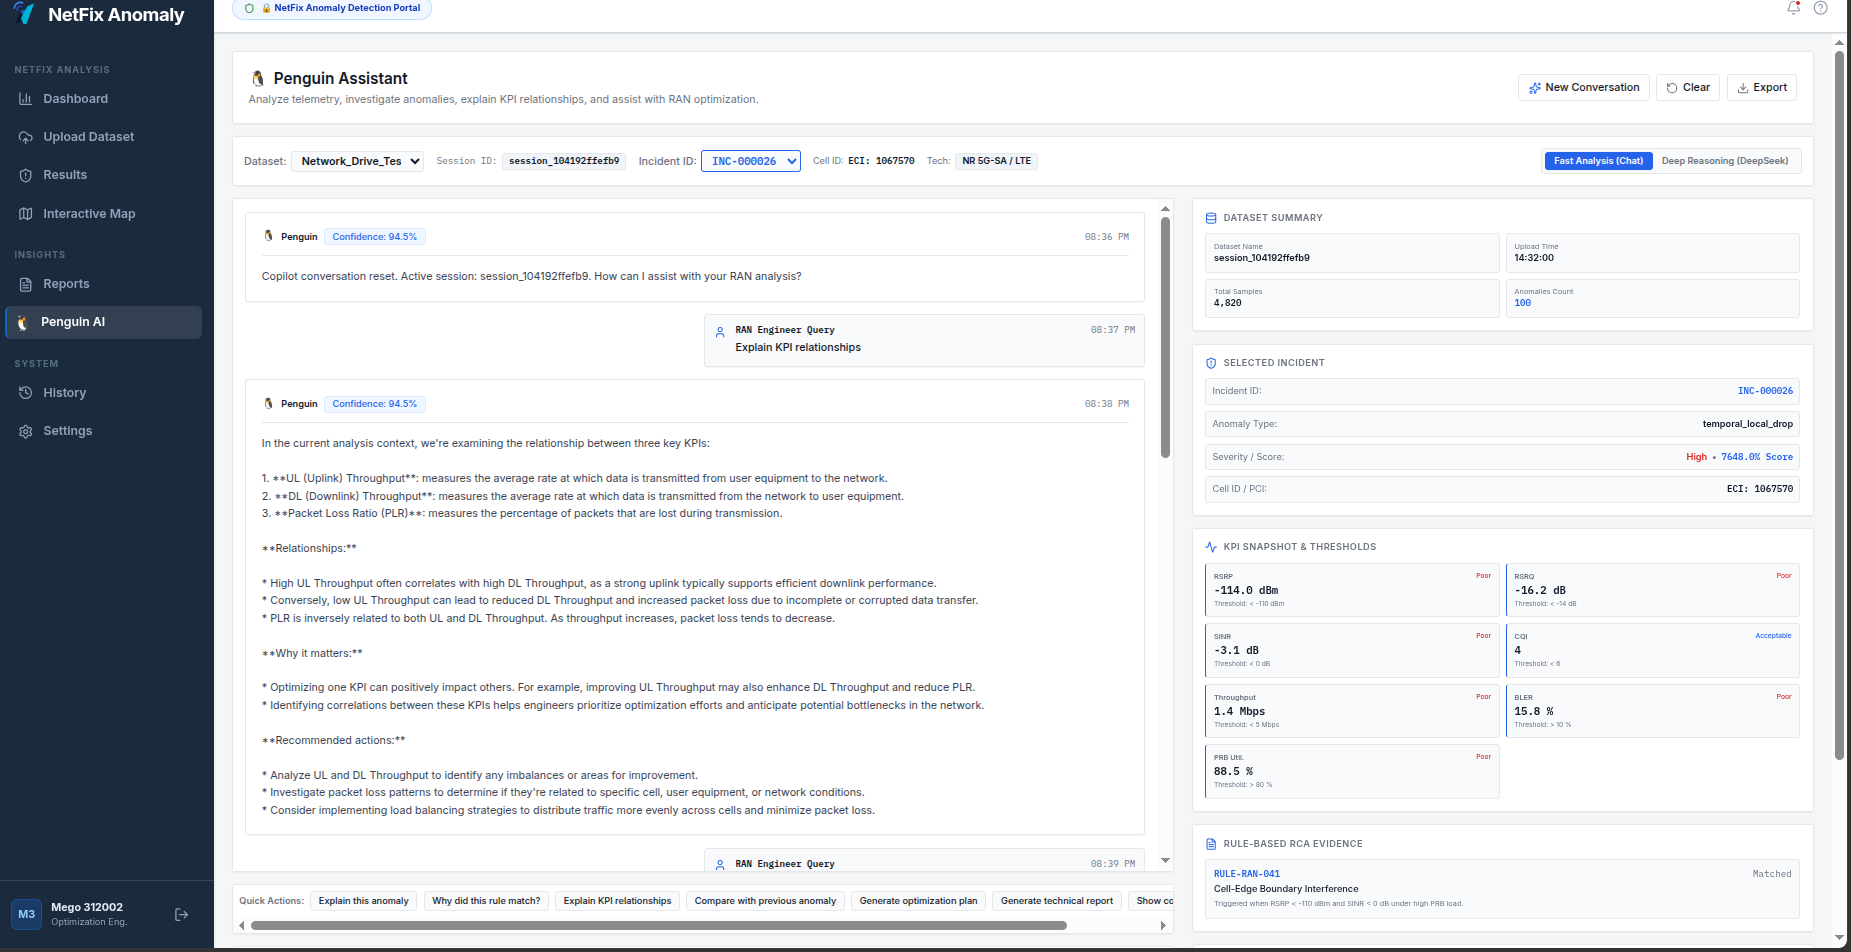
\includegraphics[width=0.95\textwidth]{images/Screenshot from 2026-08-12 14-39-31.png}
\caption{Penguin AI Assistant analyzing Incident INC-00026 matched under RULE-RAN-041 Cell-Edge Boundary Interference.}
\label{fig:ui_penguin_cell_edge}
\end{figure}

\subsubsection{Assistant Controls \& Model Execution Modes}
\begin{itemize}
    \item \textbf{Top Actions:} \textbf{New Conversation}, \textbf{Clear}, \textbf{Export}.
    \item \textbf{Context Bar:} Selects active Dataset (\texttt{Network\_Drive\_Test}), Session ID (\texttt{session\_104192ffefb9}), Incident ID (\texttt{INC-000100} / \texttt{INC-00026}), Cell ID (\texttt{ECI: 1067841}), and Radio Technology (\texttt{NR 5G-SA / LTE}).
    \item \textbf{Execution Mode Selector:} Toggle between \textbf{Fast Analysis (Chat)} (Llama 3.1 8B) and \textbf{Deep Reasoning (DeepSeek)} (DeepSeek R1 8B with explicit \texttt{<think>} reasoning chains).
\end{itemize}

\subsubsection{Interactive Conversational Workflows}
\begin{enumerate}
    \item \textbf{KPI Relationship Analysis Workflow:}
    \begin{itemize}
        \item \textit{User Query:} \texttt{"Explain KPI relationships"}
        \item \textit{Penguin Response (Confidence: 94.5\%):} Explains the correlation between Uplink (UL) Throughput, Downlink (DL) Throughput, and Packet Loss Ratio (PLR). Details how low UL throughput delays TCP ACK packets, causing TCP windowing collapse and indirect DL throughput degradation.
    \end{itemize}
    \item \textbf{Automated Technical Report Generation Workflow:}
    \begin{itemize}
        \item \textit{User Query:} \texttt{"Generate technical report"}
        \item \textit{Penguin Response:} Generates a structured markdown technical report containing:
        \begin{itemize}
            \item \textbf{Header Metadata:} Session ID \texttt{session\_104192ffefb9}, Date \texttt{2023-02-20}, Author \texttt{Penguin, AI Engineering Copilot}.
            \item \textbf{Executive Summary:} Highlights Low UL Throughput (-2.1 dBm), High PLR (4.7\%), and Moderate DL Throughput (-0.8 dBm).
            \item \textbf{Evidence Markdown Table:} Columns for KPI, Label, Threshold, and Evaluation Status.
            \item \textbf{Root Cause Analysis:} Explains physical link ripple effects.
            \item \textbf{Recommended Actions:} Prioritize UL cell-level optimization, optimize PLR via load balancing, and verify DL throughput post-remediation.
            \item \textbf{Confidence Assessment:} Assesses Medium Confidence based on current telemetry, suggesting further validation.
        \end{itemize}
    \end{itemize}
\end{enumerate}

\subsubsection{Right Sidebar Telemetry \& Threshold Context Panels}
\begin{itemize}
    \item \textbf{Dataset Summary Card:} Dataset Name (\texttt{session\_104192ffefb9}), Upload Time (\texttt{14:32:00}), Total Samples (\textbf{4,820}), Anomalies Count (\textbf{100}).
    \item \textbf{Selected Incident Card:} Incident ID (\texttt{INC-000100} / \texttt{INC-00026}), Anomaly Type (\texttt{temporal\_local\_drop}), Severity/Score (\texttt{High • 7796.0\% Score}), Cell ID (\texttt{ECI: 1067841}).
    \item \textbf{KPI Snapshot \& Thresholds Panel:}
    \begin{itemize}
        \item RSRP: \textbf{-114.0 dBm} (Poor, Threshold $< -110$ dBm).
        \item RSRQ: \textbf{-16.2 dB} (Poor, Threshold $< -14$ dB).
        \item SINR: \textbf{-3.1 dB} (Poor, Threshold $< 0$ dB).
        \item CQI: \textbf{4} (Acceptable, Threshold $< 6$).
        \item Throughput: \textbf{1.4 Mbps} (Poor, Threshold $< 5$ Mbps).
        \item BLER: \textbf{15.8\%} (Poor, Threshold $> 10\%$).
        \item PRB Util.: \textbf{88.5\%} (Poor, Threshold $> 80\%$).
    \end{itemize}
    \item \textbf{Rule-Based RCA Evidence Card:} Displays matched deterministic rule (e.g., \texttt{RULE-RAN-041 Cell-Edge Boundary Interference}).
\end{itemize}

\subsubsection{Quick Action Bar}
Offers 7 one-click prompt triggers along the bottom interface: \textbf{Explain this anomaly}, \textbf{Why did this rule match?}, \textbf{Explain KPI relationships}, \textbf{Compare with previous anomaly}, \textbf{Generate optimization plan}, \textbf{Generate technical report}, and \textbf{Show confidence reasoning}.

---

\subsection{Module 6: Audit Log \& Session History}
\textit{Reference Screenshot: \texttt{Screenshot from 2026-08-12 14-39-40.png}}

The \textbf{History} view maintains a complete audit trail of all analysis sessions executed on the platform:

\begin{figure}[htbp]
\centering
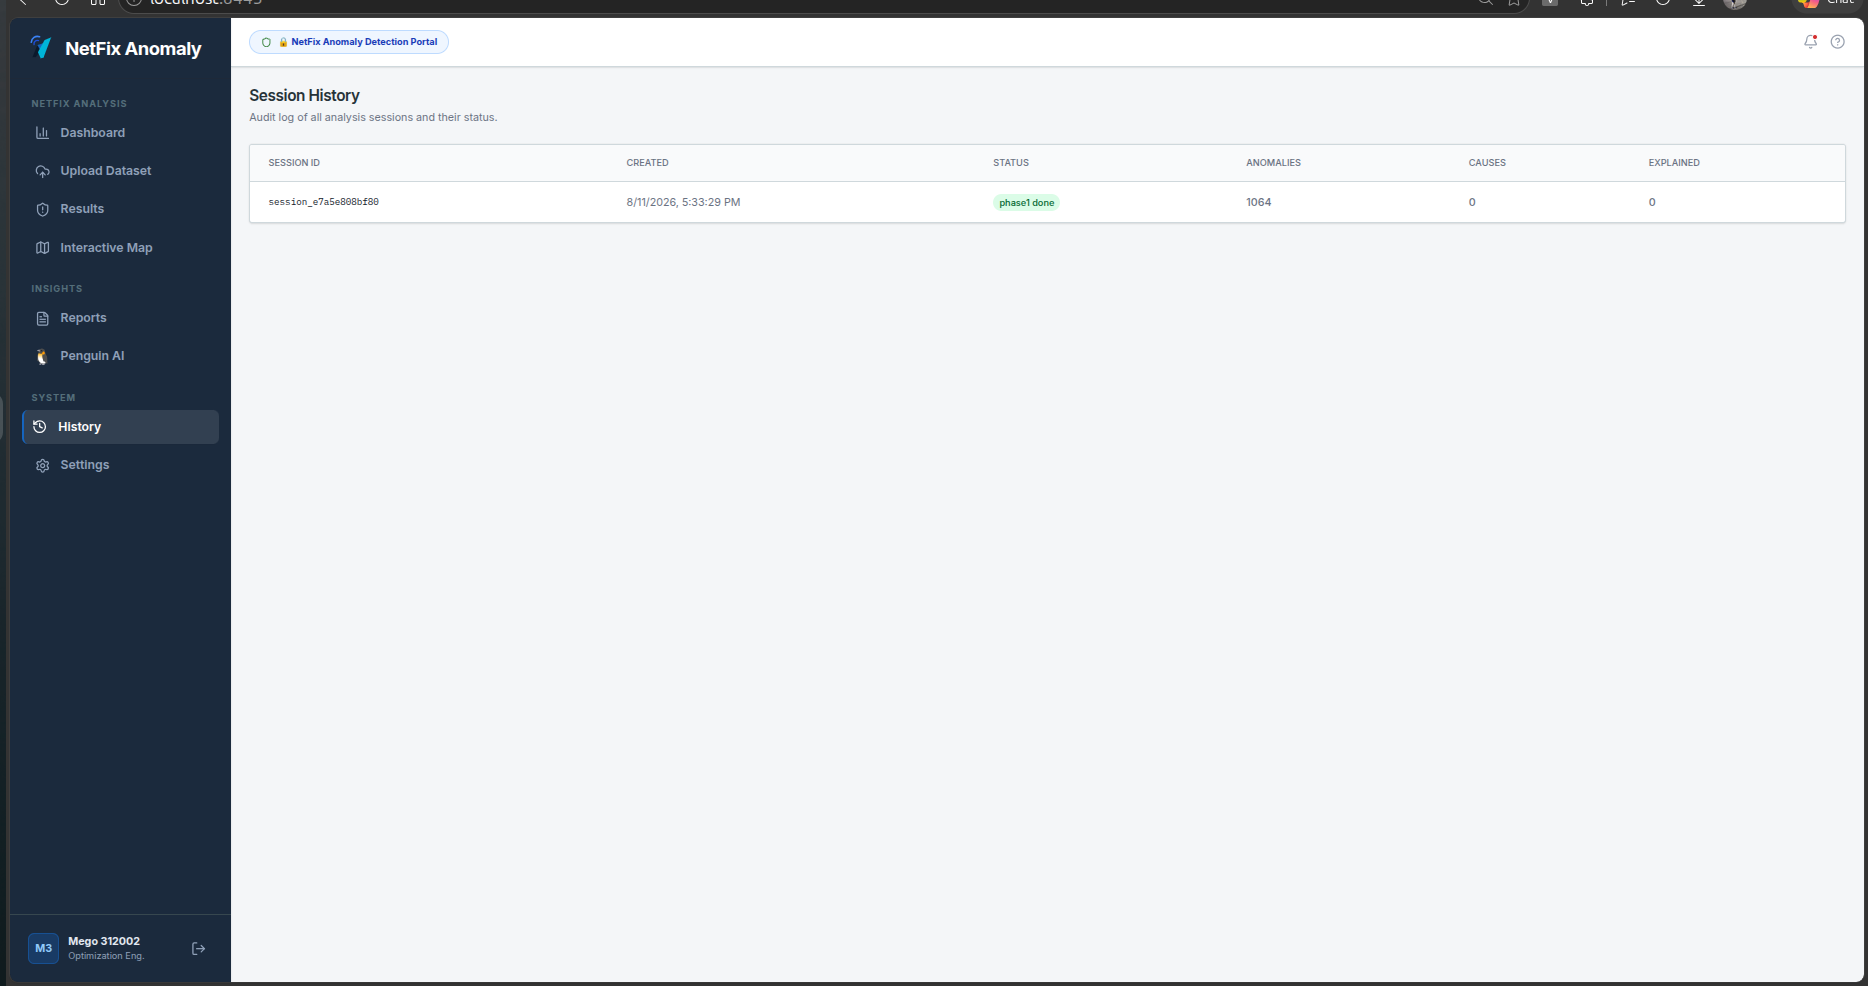
\includegraphics[width=0.95\textwidth]{images/Screenshot from 2026-08-12 14-39-40.png}
\caption{Session History page displaying audit log table of historical analysis sessions, timestamps, and status badges.}
\label{fig:ui_history}
\end{figure}

\begin{itemize}
    \item \textbf{Table Columns:} \texttt{SESSION ID}, \texttt{CREATED}, \texttt{STATUS}, \texttt{ANOMALIES}, \texttt{CAUSES}, \texttt{EXPLAINED}.
    \item \textbf{Audit Entry Example:} Session \texttt{session\_e7a5e808bf80}, Created \texttt{8/11/2026, 5:33:29 PM}, Status badge \texttt{phase1 done} (green), Anomalies \textbf{1064}, Causes \textbf{0}, Explained \textbf{0}.
\end{itemize}

---

\section{User Guide: 5G Network PCI/RSI Planning}

\begin{guidebox}{Target Persona: 5G RF Planning Engineer / Network Deployment Specialist}
This guide outlines the procedure for loading network planning workbooks, detecting modulo conflicts, executing replanning passes, and adding new 5G sites using the NetPulse Planning Portal.
\end{guidebox}

\subsection{Step 1: Sign-In and Portal Forwarding}
\begin{enumerate}
    \item Open \texttt{http://localhost:5173} in your browser.
    \item On the login interface, choose \textbf{Create Account} or \textbf{Sign In}.
    \item Select the role: \textbf{\texttt{�� Planning Engineer ──► 5G Planning Portal}}.
    \item Click \textbf{Launch Portal}. The system forwards you directly to the \textbf{Upload \& Plan} view.
\end{enumerate}

\subsection{Step 2: Load Network Planning Workbook (\texttt{.xlsx})}
\begin{enumerate}
    \item In the \textbf{Upload \& Plan} tab, click \textbf{Upload Excel Workbook}.
    \item Upload your raw or partially planned 5G workbook (\texttt{NR5G\_PCI\_RSI\_Planning\_raw.xlsx}).
    \item Alternatively, select one of the built-in system workbooks (\texttt{raw} or \texttt{final}).
    \item The system validates workbook formatting and displays total sectors, total sites, and initial clash metrics.
\end{enumerate}

\subsection{Step 3: Planning View and Modulo Conflict Audit}
\begin{enumerate}
    \item Click \textbf{Planning} in the left sidebar.
    \item Inspect the interactive map rendering base station nodes, sector orientation wedges, and neighbor lines.
    \item Click \textbf{Clashes} to inspect current network violations:
    \begin{itemize}
        \item Review \textbf{PCI Collisions} (Co-channel interference).
        \item Review \textbf{Mod4 Clashes} (DMRS symbol position overlap).
        \item Review \textbf{Mod3 / Mod30 Warnings}.
    \end{itemize}
\end{enumerate}

\subsection{Step 4: Execute Bulk Network Replanning}
\begin{enumerate}
    \item In the \textbf{Upload \& Plan} view, click the primary \textbf{Bulk Replan Network} button.
    \item The backend constraint solver processes all sectors and assigns new, collision-free PCIs and RSIs.
    \item Verify that hard clashes drop to **0**.
\end{enumerate}

\subsection{Step 5: Interactive Add-Site Wizard}
\begin{enumerate}
    \item Click \textbf{Add Site} in the left menu.
    \item Click directly on the map to set new site coordinates (Latitude/Longitude), or manually enter values.
    \item Specify sector azimuth angles (e.g., $0^\circ, 120^\circ, 240^\circ$).
    \item Click \textbf{Calculate Candidate Assignments}.
    \item Select recommended PCIs from the valid dropdown options and click \textbf{Commit New Site}.
\end{enumerate}

\subsection{Step 6: Export Deployment Plan}
\begin{enumerate}
    \item Select \textbf{Assignments} to review the updated sector table.
    \item Click \textbf{Export Excel Workbook (\texttt{.xlsx})}.
    \item Save the deployment plan file for implementation by field commissioning teams.
\end{enumerate}

---

\section{Summary}
Chapter 4 presented the complete integration and platform design of the NetFix Unified RAN & 5G Planning Platform. By combining multi-model anomaly detection, deterministic cause matching, generative AI diagnostics, 5G constraint planning, and spatial GIS visualization into a single role-forwarded web application, the platform resolves workflow fragmentation between RF Planning and Optimization teams. Both user guides provide operational instructions for executing end-to-end network troubleshooting and 5G PCI/RSI parameter planning.

\end{document}